\setcounter{footnote}{0}
\setcounter{section}{0}
\setcounter{ExNo}{0}
\begin{center}
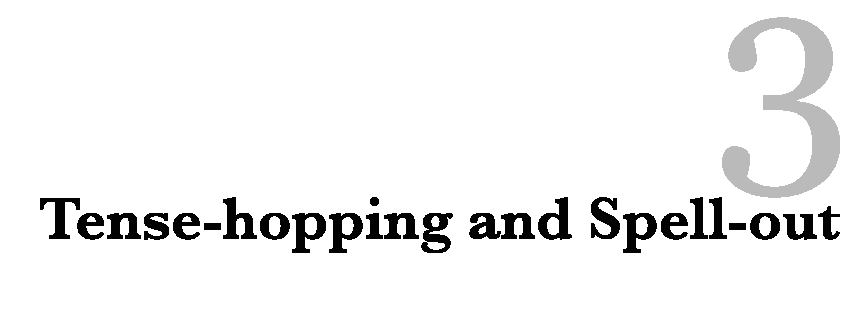
\includegraphics{chapter3.eps}
\end{center}
\section*{}
\addcontentsline{toc}{section}{\Large{Chapter 3: Tense-hopping and Spell-out}}
\section{Introduction}
In Chapter 2 I argued that Lowering, like all other syntactic transformations, is necessarily feature-driven, and, furthermore, that Lowering occurs only as a result of the \textit{Phase Head Impenetrability Condition} (PHIC). Consequently, Lowering only ever occurs to a phase head. In this chapter, we will look at another cross-linguistic phenomenon that has previously been analyzed as a case of head-to-head Lowering, namely affix-hopping of tense morphemes (\citenop{embick_noyer2001}, cf.\ \citenop{chomsky1957}, \citenop{lasnik1995}, and \citenop{ochi1999}). On the surface, it would appear that all cross-linguistic paradigms of tense-hopping meet the requirements laid out previously for Lowering transformations; e.g.\ the T head takes the \textit{v}P phase as its complement and T may carry an uninterpretable feature that is checked via a structural transformation.\footnote{\label{fn_aa}Further evidence that T may carry an uninterpretable feature comes from verb-raising languages, in which T targets the verb for upward movement. See \S\ref{verb-raising_sec} for more on verb-raising languages.} Furthermore, in all tense-hopping languages, when tense-hopping occurs, T appears adjoined to the next structurally lower overt head on the spine of the syntactic structure (i.e.\ the verb, which is contained in the complex phase head), and so has undergone a downward transformation. The null hypothesis addressed in this chapter is that all tense-hopping languages derive this pattern via the same transformational mechanism, e.g.\ head-to-head Lowering, following \citeauthor{embick_noyer2001}. In this regard, I argue in Section 2 below that not all tense-hopping patterns arise as the result of a head-to-head Lowering operation. In particular, I present evidence that, while the tense-hopping pattern of Swedish is derived via T-to-\textit{v} Lowering, tense-hopping in English occurs as a post-Vocabulary Insertion morpho-phonological merger operation under string-adjacency, i.e.\ Local Dislocation. The model presented in this section has some important implications for narrow syntactic derivation, including the nature of syntactic chains. I will argue that, when targeting an element for movement, it is not always the highest copy in a chain that is moved but rather the copy that has most recently been merged. Crucially, under a theory that allows Lowering, these two characterizations do not always apply to the same member of a chain. In Section 3, I  argue that the different patterns we observe in Swedish and English carry important consequences for a model of cyclic Spell-out----most crucially that, in the absence of Lowering, the verb and tense morphemes are spelled out on separate phases. Additionally, I discuss the exact timing of the Lowering operation, and argue for a model in which head-to-head Lowering occurs in the narrow syntactic structure rather than in the structure on the PF branch. Section 4 briefly addresses the putative T-to-C movement asymmetry in {\it wh}-questions, and Section 5 illustrates how verb-raising functions under the proposed theory. In Section 6, I summarize the chapter.\footnote{Note that the current chapter deals almost exclusively with patterns of tense-hopping. Other aspects of finite tense constructions, such as auxiliary-raising and the interaction of negation, will be dealt with in Chapter 4.}

The goal of this chapter is not simply to provide an analysis of the basic patterns of tense-hopping cross-linguistically, but rather to further develop a parsimonious model of the syntax-phonology interface that comprises the simplest architecture possible, while still making the correct predictions with a minimum of stipulations. I hope to show that so-called post-syntactic transformations should not be viewed as operations that are completely isolable from other syntactic processes, but that all stages of a derivation may be unified under a single, overarching system of linguistic computation, based primarily in the interactions of feature-checking and cyclic Spell-out operations.

\clearpage
\section{Tense-hopping: Lowering or Local Dislocation?}
As mentioned in the previous chapters, there are two theoretical possibilities for deriving the downward/rightward tense-hopping transformation under Distributed Morphology; it may either be a case of head-to-head Lowering, as in \citet{embick_noyer2001}, or a case of pre-adjunct merger Local Dislocation (i.e.\ morphological merger under PF-adjacency), as in \citet{ochi1999}. Consider again the following, which illustrates the pre-Spell-out structure of an English sentence in which tense-hopping occurs:

\singlespacing
\begin{quote}
\begin{minipage}{5.5in}
\ex. \label{Johnforget_tree} \textit{John completely forgets the address.} 

\moveleft12pt\vbox{\small{\Tree
[.TP \qroof{\{\textit{John}\}}.DP_i 
[.TP T\0\\\{\textit{\sc{pres}}\} 
[.\textit{v}P \qroof{\{\textit{completely}\}}.AP
[.\textit{v}P t_i
[.\textit{v}P [.\textit{v}\0 V\0_j\\\{\textit{forget}\}  \textit{v}  ]
[.VP t_j  \qroof{\{\textit{the address}\}}.DP 
].VP ].\textit{v}P ].\textit{v}P ].\textit{v}P ].TP ]\\}}

\end{minipage}
\end{quote}
\onehalfspacing
Under the Lowering analysis presented in Chapter 2, T in (\ref{Johnforget_tree}) would lower to \textit{v} during the Spell-out cycle of \textit{v}P as a last resort to check an uninterpretable V-feature. Under the Local Dislocation analysis, the syntactic position of T remains consistent, but the adjunct {\it completely} in (\ref{Johnforget_tree}) would not be merged until after Spell-out of the other elements. That is, the morpho-phonological string [\textit{John~$^{\wedge}$~-s~$^{\wedge}$~forget~$^{\wedge}$~the~$^{\wedge}$~address}] would be formed and Local Dislocation of tense and the verb would occur before late-merger and Spell-out of the adjunct.

In the vast majority of constructions, especially in English, these two theories make the same empirical predictions. For example, an intervening negation (e.g.\ \textit{John does not completely forget the address}) disrupts the head-complement locality requirement for T-to-\textit{v} Lowering, assuming negation in English to be an intervening non-adjunct projection. Likewise, the negation disrupts the string-adjacency requirement necessary for Local Dislocation, assuming it is not a late-merged adjunct like the {\it un-} morpheme in {\it unhappiest} (see Chapter 4, \S\ref{adjunct_block_sec}). Similarly, T-to-C movement in standard {\it yes/no} questions (e.g.\ \textit{Does John completely forget the address?}) blocks tense-hopping under both theories; under the Lowering analysis T is displaced from a position in which it takes \textit{v}P as a complement, and under Local Dislocation the phonologically overt subject, which is present even before the late merger of adjuncts, disrupts adjacency of tense and the verb; e.g.\ [\textit{-s~$^{\wedge}$~John~$^{\wedge}$~forget~$^{\wedge}$~the~$^{\wedge}$~address}].

However, these two theories do make at least one different prediction with respect to syntactic structure. In subject \textit{wh}-questions in English, tense-hopping occurs (e.g.\ \textit{Who completely forgets the address?}). Under the Lowering analysis, this indicates that T-to-C movement has not occurred, making subject \textit{wh}-questions exceptional in terms of interrogatives (compare the following object \textit{wh}-question, in which tense-hopping does not occur, indicating that T-to-C movement has taken place: \textit{What does John completely forget?}). \citet{pesetsky_torrego2001} argue that T-to-C movement indeed does not take place in subject \textit{wh}-questions. Rather, the \textit{wh}-subject, which moves to SpecCP, checks all the relevant uninterpretable features on interrogative C (see \S\ref{T-to-C_sec}). Conversely, no such T-to-C asymmetry is necessary under the Local Dislocation analysis. Movement of the \textit{wh}-subject from SpecTP to SpecCP and movement of T to C will create the initial string at Spell-out [\textit{who~$^{\wedge}$~-s~$^{\wedge}$~forget~$^{\wedge}$~the~$^{\wedge}$~address}], in which Local Dislocation of the morpho-phonologically adjacent tense and verb morphemes is licensed.

In the remainder of this section, I analyze each of these empirically adequate and theoretically possible theories of tense-hopping in more detail. I will show that a cross-linguistic analysis of tense-hopping reveals that these two theories in fact do not always make the same empirical predictions. The findings will strongly support the Local Dislocation analysis of English tense-hopping, which calls into question the necessity of positing a T-to-C movement asymmetry between subject \textit{wh}-questions and other interrogatives (to be addressed in \S\ref{T-to-C_sec}). Moreover, the model of cyclic Spell-out supported by the Lowering facts in Swedish will render a Lowering analysis of English tense-hopping untenable. As a result of these investigations, we will be able to further refine our model of the syntax-phonology interface.

\subsection{Tense-hopping cross-linguistically}
In the previous chapters, following \citet{emonds1976} and \citet{pollock1989}, I argued that a diagnostic for differentiating between tense-hopping and verb-raising languages is the general pattern of the relative positions of an inflected verb, verbal modifiers/adjuncts, and complements.\footnote{This chapter treats the verb-raising vs.\ tense-hopping distinction as a linguistic dichotomy, since we are only concerned with languages that exhibit inflected verb paradigms, as opposed to languages that encode all tense with free morphemes.} Generally speaking, standard declarative clauses in a verb-raising language exhibit the surface order [inflected~verb~$^{\wedge}$~adjunct~$^{\wedge}$~complement] (e.g.\ French) and tense-hopping languages show the order [adjunct $^{\wedge}$ inflected verb $^{\wedge}$ complement] (e.g.\ English \Last above). This is assuming a standard syntactic structure in which a discrete tense node scopes over the verb phrase, including any adjuncts to that verb phrase; e.g.\:

\singlespacing
\begin{quote}
\ex. \Tree
[.TP T\0\\bound~tense\\morpheme
[.{\it v}P \qroof{adjunct/specifier}.XP
[.{\it v}P verb \qroof{complement}.$\ldots$YP
].{\it v}P ].{\it v}P ]

\end{quote}
\onehalfspacing
Thus, in a verb-raising language the verb moves up to this tense node, past the {\it v}P-adjunct and away from its complement, whereas in a tense-hopping language the tense morpheme itself adjoins to the verb within the {\it v}P, also moving past the {\it v}P-adjunct, though in the opposite direction. As just mentioned, this tense-hopping transformation may be accounted for via either morpho-syntactic or morpho-phonological means. Differentiating between these two theories is the primary goal of this section.

We will be comparing and contrasting two tense-hopping languages, namely English and Swedish. Note that, though it is V2 in matrix clauses, the order of constituents in embedded clauses in Swedish is identical to that of English (compare the translation in \Next), where the inflected main verb follows any \textit{v}P-adjunct, showing that Swedish is also a tense-hopping language.
\\\\
\begin{minipage}{5.5in}
\singlespacing
\begin{quote}
\exg. Du vet att 	jag \textbf{ofta} \underline{l\"{a}ser} tidningen.\\
you know.\sc{pres} that I often read.\sc{pres} newspaper.\sc{def}\\
`You know that I often read the newspaper.'\\

\end{quote}
\onehalfspacing
\end{minipage}
\\In the absence of V2 head movement, which only occurs in matrix clauses in Swedish, tense morphology (e.g.\ the present tense [{\it -r}] morphology of Swedish) undergoes a downward transformation to the Swedish verb, moving past the syntactic position of the {\it v}P-adjunct. In the following section, we will see that tense-hopping also occurs in matrix clauses in Swedish, though it is often obfuscated by subsequent V2 head movement; that is, though the tense morpheme moves downward to the verb, the verb may later move higher to C, unlike in English. Taking this and other facts into consideration, I will show that Swedish and English do not derive their tense-hopping patterns via identical means, contra the null hypothesis of tense-hopping.

\subsection{\textit{v}P-fronting} \label{vp-front_sec}
Fronting of a {\it v}P that contains a matrix verb is only possible in tense-hopping languages. In verb-raising languages, the matrix verb will have moved out of {\it v}P before {\it v}P is targeted for movement. However, in tense-hopping languages, the verb remains within {\it v}P, and so will be carried along under {\it v}P-fronting. In this section, we will see that both English and Swedish allow fronting of a {\it v}P containing the matrix verb, but that a seemingly small difference in their respective patterns has crucial consequences for theories of tense-hopping, especially with respect to the Lowering vs.\ Local Dislocation debate. In particular, I argue that an asymmetry in {\it v}P-fronting strongly suggests a Lowering analysis of Swedish tense-hopping, but a Local Dislocation analysis of English tense-hopping. Additionally, the existence of this asymmetry calls into question the viability of the {\it Late Lowering Hypothesis} \citep{embick_noyer2001}, since it is argued that Lowering must be evaluated cyclically. We will also see in \S\ref{V2_sec} and Chapter 4 that this micro-variation in tense-hopping allows us to account for several other contrasting characteristics of these languages.\\

\noindent
\subsubsection{\textit{v}P-fronting in English}

\noindent
In English \textit{v}P-fronting, tense clearly does not adjoin to the verb before the \textit{v}P is moved from its original position as complement to T:

\singlespacing
\begin{quote}
\begin{minipage}{5in}
\ex. \label{En_vPfront}
\a. He said he would play the piano, and \I[vP play the piano\I]1 he did \I{\mbox{\it{t}}}1. \label{En_vPfronta} 
\b. *He said he would play the piano, and \I[vP played the piano\I]1 he (did) \I{\mbox{\it{t}}}1. \label{En_vPfrontb}

\end{minipage}
\end{quote}
\onehalfspacing
In (\ref{En_vPfronta}), the verb {\it play} appears in its uninflected form in the fronted \textit{v}P. \citet{embick_noyer2001} use these facts to argue for their \textit{Late Lowering Hypothesis} (LLH), under which Lowering does not occur until all narrow syntactic derivation has been completed. Following the LLH, tense-hopping in English, which \citeauthor{embick_noyer2001} analyze as Lowering, is not evaluated cyclically (i.e.\ on iterative Spell-out cycles to PF), but rather only after the entire narrow syntactic structure has been determined (i.e.\ on the final Spell-out cycle).\footnote{Embick and Noyer's defintion of the LLH, given the tense-hopping and \textit{v}P-fronting data, may be a bit too strong. The LLH, with respect to tense-hopping, might simply be re-stated as ``T does not lower until the Spell-out of CP.'' This would at first appear to be a reasonable assumption, given that T is first merged within the CP phase. However, we will soon see evidence that contradicts both the original LLH and this reformulation.}  As narrow syntactic \textit{v}P-fronting takes place before T-to-\textit{v} Lowering is evaluated under this analysis, and \textit{v}P-fronting displaces the verb from the complement of T, Lowering is precluded.\footnote{As noted earlier, the same holds true of T-to-C movement under a Lowering analysis, as well, since this moves T to a position in which its complement is no longer \textit{v}P.}  We will return to this issue shortly.

Under the Local Dislocation analysis of tense-hopping, the pattern in (\ref{En_vPfront}) suggests that tense and the verb are never phonologically adjacent during the course of the derivation of (\ref{En_vPfronta}). In other words, tense is not given phonological features until after \textit{v}P has been fronted in the syntax. This scenario obtains under most theories of both cyclic and non-cyclic Spell-out. For example, if T does not lower to \textit{v}P, but is rather spelled out on the CP cycle (or, alternatively, the final or only Spell-out cycle), it will not be given phonological features (i.e.\ undergo Vocabulary Insertion) until after all narrow syntactic transformations have taken place. Under a theory of cyclic Spell-out, this is due to the requirement that all narrow syntactic transformations occur before Spell-out of the matrix CP, given the \textit{Phase Impenetrability Condition} (PIC) \citep{chomsky2001}. For our purposes here, I roughly define the PIC as follows:

\singlespacing
\begin{quote}
\ex. {\it Phase Impenetrability Condition}\\
Elements embedded in the Spell-out domain of a phase $\alpha$P are not accessible to operations in a higher phase {\it \textbeta}P. 

\end{quote}
\onehalfspacing
Note that this definition is intentionally imprecise; it does not define ``Spell-out domain'' nor does it specify what constitutes an ``embedded element'', though we may assume that at least the complement of the phase head qualifies as ``embedded'' under this definition. These are issues that we will address shortly. What is important to note for now is that a consequence of the PIC is that any element that is not located at the edge of a phase $\alpha$P before Spell-out of $\alpha$P will not be able to move higher in the structure after Spell-out of $\alpha$P. At the very least, no element contained within the complement of the phase head $\alpha$ may be extracted after Spell-out of the $\alpha$P phase. In the case under consideration here, since {\it v}P is contained within the complement of C, the PIC precludes movement of {\it v}P after Spell-out of CP. Consequently, {\it v}P will move to SpecCP before phonological features are mapped to {\it in situ} T during the Spell-out cycle of CP; thus, {\it v}P is displaced before Local Dislocation of the bound tense morpheme to the verb is evaluated. Since string-adjacency of the fronted verb and {\it in situ} T does not obtain in this case, the impossibility of tense-hopping in English under the Local Dislocation analysis is likewise predicted under a theory of cyclic Spell-out.

Thus, these data in and of themselves do not support one analysis of English tense-hopping over the other, since each makes the same empirical predictions regarding the absence of tense-hopping in {\it v}P-fronting constructions. However, the Lowering analysis, with respect to the LLH, has the unfortunate drawback that it requires that transformations on the PF branch be delayed until after the narrow syntactic derivation is complete. This creates a scenario in which operations on the PF branch (e.g.\ Lowering, Vocabulary Insertion, Local Dislocation) do not occur in step with the independently motivated cyclic Spell-out operations (\citenop{chomsky2001}, \citenop{fox_pesetsky2005}, \citenop{legate2003}, \citenop{svenonius2001}, and many others). Under the most parsimonious system of cyclic Spell-out and the syntax-phonology interface, post-syntactic operations and transformations would be evaluated on each individual Spell-out cycle. This would thus derive an architecture in which morpho-syntactic structure, linearization, and phonological features of syntactic elements are all established on the same Spell-out cycles that constrain narrow syntactic derivation. Consequently, phases would be both morpho-syntactic and morpho-phonological \citep{piggott_newell2006}. In what follows, I present evidence that will lead us to conclude that such a unified system of phases is, in fact, necessary to account for certain cross-linguistic differences in tense-hopping patterns.\\

\subsubsection{\textit{v}P-fronting in Swedish}

\noindent
We have just seen that the \textit{v}P-fronting data from English do not straightforwardly allow us to choose one theory of tense-hopping over the other. However, the following data show that movement of \textit{v}P does not display an identical pattern across tense-hopping languages, which helps to shed light on the current debate. (\ref{SeV2a}) below illustrates a normal V2 word order in Swedish, in which the verb has moved to C and the DP {\it boken} has moved to the preverbal position. As we see in (\ref{SeV2b}), Swedish also moves \textit{v}P to the `preverbal' position (i.e.\ SpecCP) under \textit{v}P-topicalization. However, the verb in the fronted \textit{v}P is finite, unlike in English (examples from \citenop{kallgren_prince1989}).

\singlespacing
\begin{quote}
\begin{minipage}{5in}
\ex. \label{SeV2}
\ag.	\I[DP Boken] l\"{a}ser han nu. \label{SeV2a}\\
\hspace{1pt} book.\sc{def} read.\sc{pres} he now\\
`He is reading the book now.' \\
\bg. \I[vP L\"{a}ser boken] g\"{o}r han nu.\label{SeV2b}\\
\hspace{1pt} read.\sc{pres} book.\sc{def} do.\sc{pres} he now\\
`Reading the book he is now.' 

\end{minipage}
\end{quote}
\onehalfspacing
The fact that overt tense morphology appears on the verb in the fronted \textit{v}P is a strong indication that T adjoins to the verb in Swedish before \textit{v}P-movement occurs. Furthermore, I argue below that \textit{g\"{o}r} is a `dummy' verb, similar to \textit{do}-support in English, and that it is here a resumptive realization of a trace copy of T. This indicates that there are at least two copies of a single T head in (\ref{SeV2b}), which can only arise as the result of a morpho-syntactic transformation (e.g.\ Lowering) rather than a morpho-phonological one (e.g.\ Local Dislocation). As mentioned in Chapter 1, Local Dislocation is an adjustment to the constituency and linear order of morpho-phonological objects rather than morpho-syntactic objects. Given that Local Dislocation occurs after the point at which hierarchical syntactic structure is erased, it is unable to create traces that would be visible to subsequent structural operations, by hypothesis. Assuming that traces represent a record of the structural positions in which a syntactic element has been merged (or re-merged), Local Dislocation does not leave a trace, since this operation does not affect the syntactic, structural position of an element, but rather minimally alters the linearization scheme of the morpho-phonological representation. Lowering, on the other hand, since it operates on morpho-syntactic structure and re-merges a syntactic element in a new structural position, should indeed leave a trace, just like other head movements. Thus, the evidence strongly suggests that tense-hopping in Swedish is the result of Lowering. 

It might be tempting to analyze this asymmetry as a difference in the size of the fronted constituents; e.g.\ English fronts {\it v}Ps but Swedish fronts TPs. Note, however, that the following example shows that the fronting transformation in question is not targeting a constituent larger than \textit{v}P, given that no material in TP (neither the subject nor the modal) is fronted along with the verb phrase: 

\singlespacing
\begin{quote}
\exg. \I[vP L\"{a}sa boken] ska han.\\
\hspace{1pt} read.\sc{inf} book.\sc{def} will he\\
`Read the book, he will.'

\end{quote}
\onehalfspacing
Thus, the XP-fronting operation must be targeting a constituent smaller than TP, namely \textit{v}P.\footnote{Recall that I am assuming that V obligatorily moves to {\it v} in the languages under consideration (See Chapter 1, \S2.1). This is primarily for theoretical reasons, as the head-complement locality required for tense-to-verb Lowering does not obtain if the lexical verb remains in VP. Moreover, V2 head movement of the matrix verb requires that V move to {\it v}, as V would be subject to the PIC if it remained {\it in situ} during Spell-out of {\it v}P, thus preventing movement of the verb to C. Therefore, \Last cannot be a case of VP-fronting under this analysis, since the verb has moved out of VP.

\nobreak
I should also point out that a Local Dislocation analysis of tense-hopping makes no empirical or theoretical predictions regarding V-to-{\it v} movement. Since {\it v} is phonologically null in e.g.\ English, the same morpho-phonological string will be produced regardless of whether V raises to {\it v}. As this will not affect my analysis, I continue to assume that V raises to {\it v} in all tense-hopping and verb-raising languages.} Therefore, in example (\ref{SeV2b}), it must be the case that tense moves structurally downward into the \textit{v}P before \textit{v}P movement, which is only possible as a head-to-head Lowering operation. Given that it is a \textit{v}P constituent that is being targeted in this transformation, tense-hopping in Swedish cannot possibly be a case of Local Dislocation under any theory of Spell-out. If tense-hopping in Swedish were derived via morpho-phonological merger of the tense and verb morphemes, then both T and \textit{v} would have to be simultaneously visible and string-adjacent at PF before the {\it v}P-fronting operation occurred. If we assume non-cyclic Spell-out (i.e. there is only one Spell-out operation that occurs at the end of the derivation), then morpho-phonological adjacency of tense and the verb could not be obtained in cases of {\it v}P-fronting, as the {\it v}P would have to be fronted to SpecCP in the narrow syntax before the one-time Spell-out operation, thus disrupting the PF-adjacency of the verb and {\it in situ} T. The same restrictions hold under a model of cyclic Spell-out. If T does not lower to {\it v}, but rather remains {\it in situ} in the narrow syntax, it would only be spelled out on the matrix CP Spell-out cycle.\footnote{This is assuming, as I do throughout this thesis, that TP itself is not a phase (contra \citenop{marusic2005}). However, there is independent reason to assume this. For example, if TP were a phase, then the topicalized \textit{v}P in Swedish would necessarily have to move to SpecTP before Spell-out of TP in order to avoid a violation of the PIC, which requires that all phrases that `escape' a phase move to the edge of that phase before Spell-out (or be base-generated at the phase edge). However, if this were the case, then a Local Dislocation analysis of Swedish tense-hopping is still predicted to be impossible, as T would not be spelled out in a string-adjacent position to the verb. The {\it v}P containing the verb would be located in SpecTP when (or, at the very least, before) T is evaluated at PF (i.e.\ the structure of (\ref{SeV2}b) before TP Spell-out would be \mbox{\I[TP \I[vP \textit{l\"{a}sa boken}\I]i \I[TP \I{T}\sc{pres} \I{{\it t}}i ]]}, from which it is impossible to derive PF-adjacency of {\it l\"{a}sa} and \I{T}\sc{pres} ). Thus, I will not explore this possibility further.}  As mentioned previously, narrow syntactic extraction of \textit{v}P to SpecCP is impossible after Spell-out of CP, due to the PIC. Therefore, Swedish tense-hopping as Local Dislocation would create a timing paradox in the order of operations. The entire derivation would have to be complete (i.e.\ spelled out) before tense-hopping could occur in the matrix clause at PF, but narrow syntactic movement (e.g.\ \textit{v}P-topicalization) would have to occur after tense-hopping. We will address these issues further in the following sections, noting for now that a Lowering analysis of Swedish tense-hopping obviates the aforementioned problems, since T may lower structurally into \textit{v}P during the Spell-out cycle of \textit{v}P, and thus before derivation of CP is complete.\footnote{Note that this does not make any strong claim about whether Lowering occurs in the narrow syntactic structure or on the PF branch. However, see fn.\ \ref{narrow_syn_low_fn} and upcoming sections for a discussion of this.}

Crucially, if tense-hopping were derived via identical means in English and Swedish, we would not predict such an asymmetry in fronted \textit{v}Ps. Therefore, as tense-hopping in Swedish must be Lowering, due to the fact that the data indicate that this is a downward movement that leaves behind a trace copy, in addition to the limitations of the required order of operations, tense-hopping in English cannot be Lowering, giving us a reason to favor the pre-adjunct merger Local Dislocation analysis of English tense-hopping, as argued for by \citet{ochi1999}.

The following table summarizes this argument:
\ex. \begin{tabular}[t]{| l | l | l |}
\multicolumn{3}{c}{\textit{Possible Models of Tense-hopping}}\\\hline
 & \textbf{Late Lowering} & \textbf{Derivational Lowering}\\\hline
\textbf{Local Dislocation} & English/*Swedish & {\it English}/*Swedish\\\hline
\textbf{Lowering} & English/*Swedish & *English/{\it Swedish}\\\hline
\end{tabular}\\

The only combination that can account for all of the facts is a derivational model in which Lowering takes place during the cyclic process of syntactic derivation and tense-hopping is Lowering in Swedish and Local Dislocation in English. In the following section, we will see further evidence that supports this distinction.\\

\begin{samepage}
\subsection{Further support from V2 movement} \label{V2_sec}
In this section, I analyze V2 phenomena across languages and develop a unified approach to these patterns. I argue that, once we adopt derivational Lowering, all V2-type phenomena in Germanic languages can be explained as resulting from a [-T] feature on matrix C. This analysis will allow us to make some important claims regarding the architecture of syntactic derivations, such as a reformulation of the definition of the head of a syntactic chain---namely, the head of a chain is not necessarily the highest copy, but rather the most recently merged copy.\\

\end{samepage}

\subsubsection{Tense-attraction vs. verb-attraction}

\noindent
As shown in (\ref{SeV2a}), Swedish moves the matrix verb to verb-second position in the absence of \textit{v}P-topicalization. However, when the \textit{v}P is topicalized (\ref{SeV2b}), the inflected matrix verb appears within the fronted \textit{v}P and the semantically impoverished verb \textit{g\"{o}r} `does' appears in V2 position. I argue that this pattern allows us to make certain claims about the nature of V2 movement cross-linguistically; namely, matrix V2 head movement does not target the verb itself, but rather targets tense. The model of V2 argued for here not only supports a Lowering analysis of Swedish tense-hopping, but also reinforces a Local Dislocation analysis of English tense-hopping.

First, let us briefly look at another V2 language in order to establish a general pattern for V2 constructions. In German, like in Swedish, the inflected matrix verb in a standard declarative construction appears in verb-second position (note that I assume that German VPs and \textit{v}Ps are head-final, contra \citenop{kayne1994}):

\singlespacing
\begin{quote}
\begin{minipage}{5.5in}
\ex. \label{GeV2}
\ag. *Die Kinder den Film gesehen haben. \label{GeV2a}\\
the children the film seen have.\sc{pres}\\
\hspace{1pt}\\
\bg. Die Kinder haben den Film gesehen. \label{GeV2b}\\
the children have.\sc{pres} the film seen\\
`The children have seen the film.'\\
\cg. *Die Kinder den Film sahen. \label{GeV2c}\\
the children the film see.\sc{past}\\
\hspace{1pt}\\
\dg. Die Kinder sahen den Film. \label{GeV2d}\\
the children see.\sc{past} the film\\
`The children saw the film.'\\

\end{minipage}
\end{quote}
\onehalfspacing
Assuming that the verbs \textit{haben} in (\ref{GeV2b}) and \textit{sahen} in (\ref{GeV2d}) have undergone \textit{v}-to-T-to-C movement (\citenop{schwartz_vikner1996}, \citenop{vikner1995}, cf.\ \citenop{travis1984}, \citeyear{travis1986}, \citeyear{travis1991}), there are two possible-feature based scenarios under which this movement is derived:

\singlespacing
\begin{quote}
\begin{minipage}{5in}
\ex. \label{V2possibilities}
\a.\textit{Verb attraction} \label{V2possibilitiesa}\\
C directly targets the verb for movement to V2 position (i.e.\ C\raisebox{-3pt}{\footnotesize{[{\it -v}]}}).\footnotemark\\ 
\b. \textit{Tense attraction} \label{V2possibilitiesb}\\
C targets T for movement to V2 position; an independent head movement operation creates a complex \textit{v}+T head before C is merged, and so the verb is raised, as well, during T-to-C movement (i.e.\ C\raisebox{-3pt}{\footnotesize{[-T]}}).\\

\end{minipage}
\end{quote}
\footnotetext{I assume that all heads in the functional domain that raise verbs target a \textit{v}-feature, given the PHIC. See the later section on verb-raising languages.}
\onehalfspacing
In German, it is difficult to either prove or disprove either of the possibilities in (\ref{V2possibilities}). However, in order for (\ref{V2possibilitiesb}) to be a viable candidate, independent evidence is needed to show that the verb moves to T in non-V2 environments in German, e.g.\ embedded clauses. Assuming that TP in German, like \textit{v}P, is head-final, this is also difficult to show. Consider the following possible structure of an embedded clause in German:

\singlespacing
\begin{quote}
\begin{minipage}{5.5in}
\ex. \label{Ge_embedded_tree}
\ag. Ich weiss, [ dass die Kinder den Film sahen]. \label{Ge_embedded_treea}\\
I know.\sc{pres} [ that the children the film see.\sc{past}]\\
`I know that the children saw the film.'\\
\b. Ich weiss ... \label{Ge_embedded_treeb}

\Tree
[.CP C\0\\\{\textit{dass}\}
[.TP \qroof{\{\textit{die Kinder}\}}.DP
[.TP [.\textit{v}P \qroof{\{\textit{den Film t_i}\}}.VP [.\textit{v}\0 V\0_i\\\{\textit{sahen}\} \textit{v} ] ] T\0\\\{\textit{\sc{pres}}\}
].TP ].TP ] 

\end{minipage}
\end{quote}
\onehalfspacing
In (\ref{Ge_embedded_treeb}), since there is never a structural intervener between the syntactic positions of {\it v} and T (e.g.\ an adjunct that is unquestionably right-adjoined to {\it v}P), there is no straightforward structural way to determine whether string-vacuous movement of \textit{v} to T occurs. \citet{schwartz_vikner1996} argue, however, that {\it v} does raise to T in German. Their argument is based primarily on the richness of inflection of German verbs. Many analyses (e.g.\ \citenop{bobaljik2000b}, \citenop{holmberg_platzack1995}) have argued for a correlation between verb-raising and a rich system of verbal morphology. It has been observed that languages that exhibit \textit{v}-to-T movement (e.g.\ Italian, French) tend to have a more varied paradigm of verbal inflection than tense-hopping languages (e.g.\ English, Swedish).\footnote{See \S\ref{rich_agr_sec} for further investigation into the Rich Agreement Hypothesis.}  Note that German displays a much richer inflectional paradigm than Swedish or English:

\singlespacing
\begin{quote}
\begin{minipage}{5in}
\ex.
\raisebox{-.6in}{\begin{tabular}{lclcl}
\underline{German}&vs.&\underline{Swedish}&vs.&\underline{English}\\
ich nehme&&jag tar&&`I take'\\
du nimmst&&du tar&&`you(sg) take'\\
er nimmt&&han tar&&`he takes'\\
wir nehmen&&vi tar&&`we take'\\
ihr nehmt&&ni tar&&`you(pl) take'\\
sie nehmen&&de tar&&`they take'\\
\end{tabular}}

\end{minipage}\\
\end{quote}
\onehalfspacing
While this does not provide irrefutable proof that \textit{v} independently raises to T in German, it does allow us to entertain the possibility that the tense-attraction analysis of V2 movement is the correct one.\footnotemark \footnotetext{Note that if \textit{v} does not raise to T in German, then German is also a tense-hopping language, as the verb in the embedded clause carries finite tense morphology. There is no strong empirical evidence to suggest that this is or isn't the case, however. Also, see the appendix to this chapter on the possibility of matrix {\it v}P-fronting in certain registers of German.} Furthermore, as we will see below, this analysis allows for a more uniform system of V2 phenomena cross-linguistically.\\

\subsubsection{Derivational vs.\ representational syntactic chains}\label{deriv_rep_chains_sec}
I have argued that T lowers to {\it v} cyclically in Swedish. This raises a new theoretical question: when a higher head merges and probes a chain that contains a lowered head, which copy in that chain is targeted for movement? I believe the answer to this question allows us to derive the V2 head pattern straightforwardly in Swedish. As noted above, we will assume the tense-attraction analysis of V2. Recall, however, that unlike the proposed scenario for German, verbs do not raise to T in Swedish---evidenced by the fact that Swedish allows fronting of a {\it v}P containing the matrix verb--, yet T-to-C V2 movement still targets the verb and tense as a single syntactic constituent, as shown in (\ref{SeV2a}), repeated in \Next below, in which the inflected verb {\it l\"{a}ser} occupies the C/V2 position.

\singlespacing
\begin{quote}
\begin{minipage}{5in}
\exg. \label{SeV2_repeata}
\I[DP Boken] l\"{a}ser han nu.\\
\hspace{1pt} \hspace{1pt} book.\sc{def} read.\sc{pres} he now\\
`He is reading the book now.' \\

\end{minipage}
\end{quote}
\onehalfspacing
This pattern is explained if T undergoes Lowering to \textit{v} before C merges into the narrow syntactic derivation and targets T for movement; since Lowering of tense is a syntactic head-to-head movement, it forms a complex syntactic object containing both T and \textit{v}. I claim that, with a slight modification to our view of derivational probing operations and syntactic chains (see below), T-to-C V2 movement will target the complex T+\textit{v} structure formed via Lowering, when possible (i.e.\ when the inflected verb is still within the c-command domain of C when T-to-C movement is evaluated, which is the case in the absence of \textit{v}P-fronting; see below).\footnote{\label{narrow_syn_low_fn}Since the complex {\it v}+T head is visible to higher heads, this analysis suggests that the Lowering operation occurs in the narrow syntax, rather than solely on the PF branch. I return to this issue in later sections, where I compare and contrast a theory of Lowering on the PF branch with a theory of Lowering in the narrow syntax. While both models are theoretically possible, we will ultimately see that the narrow syntactic theory of Lowering is the less problematic of the two options. Crucially, however, I will continue to argue that Lowering is motivated by Spell-out operations, and is thus closely linked with the process of assigning phonological form to syntactic structures. It is important to note for now only that a Lowering operation creates a complex morpho-syntactic {\it v}+T head at some point of the derivation, and that this complex head becomes targetable for T-to-C V2 movement.} I propose that the following is the (rough) structure of \Last at the point at which T-to-C V2 movement is evaluated (see \S\ref{loc_low_sec} for a step-by-step derivation of this structure, in which I illustrate that tense-lowering occurs before C is merged into the derivation; note also that I will later address the timing of phrasal versus head movement in the V2 pattern):

\singlespacing
\begin{quote}
\begin{minipage}{5in}
\ex. \textit{Boken l\"{a}ser han nu.} \label{SeV2DP_tree}

\Tree
[.CP \qroof{\{\textit{boken}\}}.DP_i
[.CP C\raisebox{-4pt}{\footnotesize{[-T]}}
[.TP \qroof{\{\textit{han}\}}.DP
[.TP \sout{T}_j\\\{\sc{\sout{pres}}\} \qroof{\textit{l\"{a}sa+}\mbox{\sc{pres}_j} \textit{t_i\ nu}}.\textit{v}P
].TP ].TP ].CP ] 

\end{minipage}\\
\end{quote}
\onehalfspacing
In (\ref{SeV2DP_tree}), the trace of T created via Lowering forms a chain with the derivationally most recent copy on \textit{v} adjoined to {\it l\"{a}sa}, since the trace c-commands the lower copy. I argue that when T-to-C movement is evaluated, C does not target the structurally closest copy of T (i.e.\ the trace of T in TP), but rather targets the lower copy adjoined to {\it v}. Thus, when C probes for T, it targets the most recent copy of T and raises the \textit{v}+T (i.e.\ {\it l\"{a}sa+}\mbox{\sc{pres}}) head to V2 position.\footnote{Recall that, as mentioned in Chapter 2, there is no \textit{a priori} reason to think that movement through a trace of a lowered head is impossible.}

Crucially, it is not the structurally highest copy of T that is targeted for movement in \Last. This analysis entails an important revision to the notion of ``syntactic chains'', since, traditionally, it is the structurally highest copy in a chain that is targeted for movement. Under this traditional view, a head Y that probes an element X will always target the closest (i.e.\ highest) copy of X found in the syntactic representation when Y is merged. However, I argue that syntactic chains are purely derivational, rather than representational. While I maintain that all members of a chain must be in a c-command relation (i.e.\ a chain consists only of copies that c-command or are c-commanded by another copy of themselves),\footnote{See \citet{epstein_etal1998} and \citet{kawashima_kitahara1996} for a derivational view of c-command relations.} I adopt the following definition of the head of a syntactic chain:

\begin{samepage}
\singlespacing
\begin{quote}
\ex. {\it Head of chain (derivational):} \label{head_chain_def} \\
In a syntactic chain C\raisebox{-3pt}{\mbox{\sc{h}}}, where C\raisebox{-3pt}{\mbox{\sc{h}}} = \{$\alpha_{i} \ldots\alpha_{i}\ldots$\}, $\lvert$C\raisebox{-3pt}{\mbox{\sc{h}}}$\rvert$~$>$~1, and each $\alpha$ is a copy of \textit{\textbeta}\ that c-commands and/or is c-commanded by another copy of \textit{\textbeta}, the head of C\raisebox{-3pt}{\mbox{\sc{h}}} is the $\alpha$ that was most recently merged into the derivation.\footnotemark

\end{quote}
\footnotetext{If $\lvert$C\raisebox{-3pt}{\mbox{\sc{h}}}$\rvert$~$=$~1, then the single member of C\raisebox{-3pt}{\mbox{\sc{h}}} is vacuously the head of C\raisebox{-3pt}{\mbox{\sc{h}}}.}

\end{samepage}
\onehalfspacing
\noindent
Under \Last, the head of the chain created by Lowering of T in \LLast is the copy contained within the {\it v}P, rather than the copy that is structurally highest (i.e.\ the copy in the base position of T). I argue that it is the head of this chain---under the above definition---that is targeted in feature-probing operations. Thus, in all probing operations, the probing head targets (or attempts to target) the most derivationally recent copy of the targeted constituent.\footnote{See below for an analysis of ``broken chains'', i.e.\ cases in which the derivationally most recent copy is inaccessible to a probing head.} In the absence of Lowering, the most recent copy within a targeted chain will invariably be the structurally highest copy. In other words, in cases in which all syntactic transformations proceed as raising operations (i.e.\ re-merger of a copy to a structurally higher position), all trace copies within a chain will be found in a structurally lower position than the derivationally most recent copy, and so the head of the chain will be the highest copy; e.g.\ (numeric subscripts on `X' indicate the order in which each copy is merged/re-merged):\footnote{I limit myself to head movement here, though the same claims hold for phrasal movement.}$^{,}$\footnote{All elements in \Next are contained within the same Spell-out domain; see \S\ref{Low_cyclic_sec}.}

\singlespacing
\begin{quote}
\ex. Raising\\
\Tree
[.ZP [.Z\0 [.Y\0 \node{3}{X$_{3}$\0} Y ].Y\0 Z\raisebox{-3pt}{\footnotesize{[-X]}} ]
[.YP [.Y\0 \node{2}{X$_{2}$\0} Y\raisebox{-3pt}{\footnotesize{[-X]}} ]
[.XP \node{1}{X$_{1}$\0} \qroof{$\ldots$}.WP
].XP ].YP ]
\anodecurve[bl]{1}[b]{2}{.5in}
\anodecurve[bl]{2}[b]{3}{.5in}

\end{quote}
\onehalfspacing
In \Last, upward head movement transformations have created three copies of X. After the first head movement, the chain \{X$_{2}$, X$_{1}$\} is created, where the order of elements indicates a c-command relation (i.e.\ X$_{2}$ c-commands X$_{1}$). When Z$^{0}$\raisebox{-3pt}{\footnotesize{[-X]}} merges and targets X for movement, X$_{2}$ is both the derivationally most recent and the structurally highest copy of X, and it is targeted for movement to Z$^{0}$ (pied-piping Y$^{0}$ in the process), creating the chain \{X$_{3}$,~X$_{2}$,~X$_{1}$\}. In this chain, X$_{3}$ is now the head, under either a representational or derivational definition of ``head of chain'', and so will be targeted in any subsequent transformations of X to a higher head.

However, when Lowering occurs, it is not immediately obvious which copy will qualify as the head of the resulting chain; e.g.:\footnote{X and Y in \Next are merged in separate Spell-out domains; see \S\ref{Low_cyclic_sec}.}

\singlespacing
\begin{quote}
\ex. Lowering\\
\Tree
[.XP \node{4}{X$_{1}$\0}\raisebox{-3pt}{\footnotesize{[-W]}}
[.YP [.Y\0 [.W\0 \node{5}{X$_{2}$\0} W ].W\0 Y ] \qroof{$\ldots$}.WP
].YP ]
\anodecurve[bl]{4}[bl]{5}{.5in}\\

\end{quote}
\onehalfspacing
Lowering of X in \Last creates the chain \{X$_{1}$, X$_{2}$\}. However, X$_{1}$ is the structurally highest copy, while X$_{2}$ is the derivationally most recent copy. When compared with the raising example in \LLast, we see that a distinction between ``structurally highest copy'' and ``derivationally most recent copy'' only arises in such cases of Lowering. Given that the matrix verb in Swedish is moved to C in standard V2 movement (and interrogatives; see below), we can maintain a tense-attraction (i.e.\ T-to-C) analysis of V2 head movement by adopting the revised definition of ``head of chain'' as the most recent, rather than the highest, copy in a chain. In a tense-hopping language like Swedish, finite T invariably lowers to {\it v}. If and when C\raisebox{-3pt}{\footnotesize{[-T]}} merges, it targets the head of the T chain (where possible; see below), which, at this point in the derivation, is the copy adjoined to the verb in {\it v}P, and so the verb is carried along in the T-to-C transformation.\footnote{Although the lowered T head has undergone Spell-out and is thus embedded in the phase head, I argue in \S\ref{loc_low_sec}  that it may still be targeted for movement by virtue of the fact that a higher element in its well-formed chain (i.e.\ the trace of T) is still visible to higher elements (see esp. fn.\ \ref{phase_chain_fn}).}

Computationally speaking, I believe this to be a conceptually desirable model of syntactic chains and derivations. Under the simple view of syntactic derivation as a process that manipulates individual elements from a numeration, combining and re-combining those elements in principled ways, it is the copy of each individual element which has most recently been manipulated by the computational component that is active in the on-line derivation. Syntactic transformations consist of moving an element from one position to a new position derivationally, i.e.\ in a step-wise fashion. As mentioned earlier, trace copies represent the derivational history of a particular syntactic element; that is, traces show where an element has been, rather than where it is currently at a given point of the derivation. However, I argue that on-line derivation should be most sensitive to the most recent copies of the elements involved---i.e.\ the current locations of those elements--, rather than ``looking back'' to the historical positions of a given element.\footnote{Note that I say ``most sensitive'' since it is possible for traces to be targeted in transformations when the derivationally most recent copy is inaccessible; see below.} Thus, whenever possible, a syntactic transformation will target the most recently active copy (i.e.\ the most recently merged copy) in a derivation, instead of targeting a derivationally ``older'' copy, i.e.\ a trace. This reduces the computational burden on syntactic derivation, since, all things being equal, the most economical derivation will simply continue the progressive movement of an active copy. A consequence of this is that, under most circumstances, trace copies within a chain are derivationally inert, regardless of their position with respect to the most derivationally recent copy.\footnote{As pointed out by Lisa Travis (p.c.), this treats syntactic objects as ``real'' objects. When looking for a real object, you target its last known position.} We return to this in a moment.

The following summarizes the effects of this model for standard V2 movement in Swedish:

\singlespacing
\begin{samepage}
\begin{itemize}
\item Finite T undergoes head-to-head Lowering to {\it v} in both matrix and embedded clauses in Swedish, leaving a trace copy of T in TP.
\item If and when C\raisebox{-3pt}{\footnotesize{[-T]}} merges, it will target the derivationally most recent copy of T if that copy is contained in its c-command domain (see below).
\item As the derivationally most recent copy of T is adjoined to the verb, the verb will be pied-piped in T-to-C V2 (and interrogative; see \S\ref{V2_sec}.5) movement.

\end{itemize}
\end{samepage}
\onehalfspacing
This therefore allows for movement of the main verb to V2 position in a tense-lowering language like Swedish under a tense-attraction analysis of V2 constructions. As noted previously, a Local Dislocation analysis of tense-hopping is incapable of creating a morpho-syntactic {\it v}+T constituent at any level of the derivation, as Local Dislocation creates complex morpho-phonological, rather than morpho-syntactic, objects. Since {\it v}+T is targeted as a morpho-syntactic constituent in T-to-C movements, under the proposed model, we have further support for a Lowering analysis of Swedish tense-hopping.\\

\subsubsection{Timing of V2, re-merger of trace copies, and ``stowaway'' movement}

\noindent
We can now also explain the presence of the `dummy' verb \textit{g\"{o}ra} in Swedish \textit{v}P-topicalization. Recall that in (\ref{SeV2b}), repeated in \Next below, the matrix verb is contained in the fronted \textit{v}P, and the V2 position is occupied by the semantically impoverished verb \textit{g\"{o}r}:

\singlespacing
\begin{quote}
\begin{minipage}{5.5in}
\exg. \I[vP L\"{a}ser boken] g\"{o}r han nu.\label{SeV2_repeatb}\\
\hspace{1pt} read.\sc{pres} book.\sc{def} do.\sc{pres} he now\\
`Reading the book he is now.' 

\end{minipage}
\end{quote}
\onehalfspacing
Furthermore, the tense on the verb \textit{g\"{o}ra} must be identical to the tense on the verb in the fronted \textit{v}P, suggesting that these overt tense morphemes are two copies of a single T head (examples from \citenop{kallgren_prince1989}, ex. (4)).\\

\singlespacing
\begin{quote}
\begin{minipage}{5.5in}
\ex. \label{SeTIdent}
\ag. *\I[vP L\"{a}ser boken] gjorde han. \label{SeTIdenta}\\
\hspace{1pt} read.\mbox{\sc{pres}} book.\mbox{\sc{def}} do.\mbox{\sc{past}} he\\
\bg. \I[vP L\"{a}ste boken] gjorde han. \label{SeTIdentb}\\
\hspace{1pt} read.\sc{past} book.\sc{def} do.\sc{past} he\\

\end{minipage}
\end{quote}
\onehalfspacing
I therefore assume, and argue further below, that the form of {\it g\"{o}ra} present in \LLast and \Last[b] is a resumptive pronunciation of a trace copy of T, and that these examples therefore have only one lexical verb, {\it l\"{a}sa}. This has an immediate consequence for the timing of V2 head and phrasal movements. Namely, \textit{v}P must move to SpecCP before T-to-C V2 head movement is evaluated. This must hold under any theory of V2 movement (e.g.\ tense-attraction or verb-attraction); if the \textit{v}P were \textit{in situ} when head movement to C is evaluated, then any model of V2 movement would predict that the \textit{v}+T constituent would be moved to C, like in other V2 constructions in Swedish. Subsequently, the \textit{v}P containing just the direct object \textit{boken} in (\ref{SeV2_repeatb}) would undergo remnant movement to SpecCP (see fn. \ref{fn_remnant_mov}), making it indistinguishable from (\ref{SeV2_repeata}); e.g.\ [\I[vP t$_{i}$~boken]$_{k}$~l\"{a}ser$_{i}$~han~t$_{k}$~nu]. Therefore, it must be the case that the verb (or, more appropriately, the most recent copy of T that is adjoined to the verb) is not within the c-command domain of C when V2 head movement is evaluated. This is derived only if XP movement to C happens before head movement to C, since the verb contained within {\it v}P must escape the syntactic environment in which it is an appropriate target for V2 head movement to C. Further research is needed as to why this is the case. However, such an investigation would take us far afield from our current concern with downward transformations, and so I leave this as an open question. I note for now that the only problem this model immediately poses is that it violates the Extension Condition, in that a head movement to X that follows a phrasal movement to SpecXP is targeting a non-root position. However, as mentioned briefly in Chapter 1, head movement in general faces this same dilemma, and so I do not believe that this constitutes a serious objection to this order of movement operations. We will thus assume from now on that {\it v}P in Swedish {\it v}P-topicalization moves to SpecCP before V2 head movement to C is evaluated.

Taking the above into consideration, it is therefore the case that in the \textit{v}P movement examples (\ref{SeV2_repeatb}) and (\ref{SeTIdentb}), unlike in the \textit{v}P-\textit{in situ} example (\ref{SeV2_repeata}), the active (i.e.\ the derivationally most recent) copy of T is no longer contained within the c-command domain of C when C probes for T. In (\ref{SeV2_repeatb}) and (\ref{SeTIdentb}), the {\it v}P containing the {\it v}+T constituent has already been fronted before head movement to C is evaluated, and so the active copy of T is found in SpecCP, where it cannot be a goal for the probing C head. In other words, the tense chain has been ``broken''. Therefore, I argue that since the derivationally active copy of T cannot be targeted for movement to C, but C must still satisfy its [-T] feature, C instead targets an intermediate copy of T for V2 movement, which will be realized phonologically via `do'/{\it g\"{o}ra}-support. I argue that this is a type of syntactic repair mechanism which occurs when only trace copies of the targeted element are found in the c-command domain of the probing head. This is formalized as follows:

\singlespacing
\begin{quote}
\ex. {\it Trace re-merger}\\
When a head $\alpha$ probes for a feature [$\beta$], it targets the active (i.e.\ the most recently created) copy of a syntactic element $\gamma$ carrying [$\beta$]. If the active copy of $\gamma$$_{[\beta]}$ is not contained within the c-command domain of $\alpha$, $\alpha$ targets the closest copy of $\gamma$$_{[\beta]}$.

\end{quote}
\onehalfspacing
I'll first illustrate how \Last accounts for the Swedish pattern, and then discuss some of its consequences. The pattern in Swedish {\it v}P-fronting arises as the result of the second clause in \Last, since, as mentioned above, the active copy of T is found in SpecCP when C probes for T. We begin with the structure for (\ref{SeV2_repeatb}) at the point at which T-to-C V2 movement is evaluated.\footnote{Note that the adverb \textit{nu} `now' is omitted from this representation for clarity. It may either be an adjunct to TP or a late-merged adjunct to the trace of \textit{v}P. However, this is not crucial for the current analysis.}$^{,}$\footnote{Although there is a copy of T that is found in the lower copy of {\it v}P in \Next, as a result of T-to-{\it v} Lowering, it is not the active copy, nor is it the closest copy to C. Therefore, following \Last, this copy is not targeted for movement.} 

\singlespacing
\begin{quote}
\begin{minipage}{5.5in}
\ex. \textit{L\"{a}ser boken g\"{o}r han nu.} \label{SeV2vP_tree}

\Tree
[.CP \qroof{\{\textit{l\"{a}sa+\mbox{\sc{pres}_j} boken}\}}.\textit{v}P_i
[.CP C\raisebox{-4pt}{\footnotesize{[-T]}}
[.TP \qroof{\{\textit{han}\}}.DP
[.TP \sout{T}_j\\\{\sc{\sout{pres}}\} \qroof{...}.\sout{\textit{v}P_i}
].TP ].TP ].CP ] 

\end{minipage}
\end{quote}
\onehalfspacing
In (\ref{SeV2vP_tree}), the T head has lowered (i.e.\ re-merged) to the head of \textit{v}P, which contains the verb root {\it l\"{a}sa}. The \textit{v}P is later fronted to SpecCP. We may call this ``stowaway'' movement (Lisa Travis, p.c.), since a head X moves into a phrase YP before that YP is targeted for movement. The YP therefore carries along its ``stowed away'' passenger X.\footnote{Note that this is quite different from ``smuggling'' \citep{collins2005}. In smuggling, a phrase YP contains an element X. However, X cannot be accessed by a higher constituent Z in its base position due to e.g.\ relativized minimality considerations. Licit movement of YP to a higher position may ``smuggle'' X to a position from which it may be accessed by Z. The primary difference between ``stowaway'' and ``smuggling'' movement is that in stowaway movement, X is generated outside of YP and moves into YP before YP is targeted for movement; in smuggling, X is base-generated within YP and only moves out of YP after movement of YP. See also fn. \ref{fn_remnant_mov} for a comparison of stowaway and remnant movement.} After the stowaway movement process of T-to-{\it v} Lowering followed by {\it v}P-fronting, head movement to satisfy the V2 requirement is evaluated. We see here that, crucially, the active copy of T, which is contained within the fronted \textit{v}P (i.e.\ the stowed away copy of T), is no longer within the c-command domain of C. Therefore, since the active copy is not targetable by C, unlike when \textit{v}P remains \textit{in situ}, C targets the closest trace copy of T that it c-commands for T-to-C movement, re-merging another copy of T in the C head to check C's [-T] feature, as follows:\footnote{The copies of T that are not represented with \sout{strikethrough} are those that are pronounced; see the following discussion.} 

\singlespacing
\begin{quote}
\begin{minipage}{5.5in}
\ex. \textit{L\"{a}ser boken g\"{o}r han nu.} \label{SeV2vP_Tmov_tree}

\Tree
[.CP \qroof{\{\textit{l\"{a}sa+\mbox{\sc{pres}_j} boken}\}}.\textit{v}P_i
[.CP C+T_j\\\{\sc{pres}\}
[.TP \qroof{\{\textit{han}\}}.DP
[.TP \sout{T}_j\\\{\sc{\sout{pres}}\} \qroof{...}.\sout{\textit{v}P_i}
].TP ].TP ].CP ] 

\end{minipage}
\end{quote}
\onehalfspacing
Note that we now have a ``broken'' tense chain. Stowaway movement of T via T-to-{\it v} Lowering and {\it v}P-fronting to SpecCP has created two chains for the \mbox{\{\sc{pres}\}} head; one that contains a single member that is found in the fronted \textit{v}P (i.e.\ this copy does not c-command any other copy of \mbox{\{\sc{pres}\}}, nor is it c-commaned by another copy, and so it is vacuously the head of its chain), and another that is headed by the copy in C (i.e.\ given the proposed order of operations, the copy of T in C is now the active copy in this chain). As all movement represented in (\ref{SeV2vP_tree})-(\ref{SeV2vP_Tmov_tree}) is overt, I propose that the head of each \mbox{\{\sc{pres}\}} chain is pronounced, as is argued to be the case with all PF chains (\citenop{bobaljik1995}, \citenop{groat_oneil1996}, \citenop{nissenbaum2000}).\footnote{\label{fn_remnant_mov}Note that this stowaway movement is the structural inverse of remnant movement. Under remnant movement, an element is raised out of an XP before that XP is targeted for movement, whereas in stowaway movement an element, namely T, is lowered into an XP before that XP is moved. \citet{muller1998} proposes a \textit{Proper Chain-Binding Condition} (PCBC), which requires that the trace of a remnant-moved XP be c-commanded by the antecedent of any trace within that XP. That is, an element Y that has been moved out of XP before XP moves higher must bind the trace of XP. However, in the Swedish \textit{v}P-topicalization cases of stowaway movement, the copy of T contained within the fronted \textit{v}P does not bind any trace of itself or a constituent in which it was once contained. Therefore, at PF interpretation, no chain whatsoever can be formed between the fronted copy of T and its trace copies. My proposal is simply that, 1) since the fronted copy does not form any sort of chain with other copies of T, it is pronounced, and 2) the head of the chain of trace copies in C and the base position of T is likewise pronounced.}$^{,}$\footnote{In the case of embedded clauses in Swedish, it is the copy of T found on the {\it in situ} verb---i.e.\ below the base position of T--, that is pronounced. Thus, the definition of ``head of chain'' in (\ref{head_chain_def}) holds for these pronunciation facts, as well, since it is the copy of T found on the verb that is the active copy in this chain.}  Since the head of the second chain contains only the bound morpheme \mbox{\{\sc{pres}\}}, the dummy verb \textit{g\"{o}ra} `do' is inserted, akin to \textit{do}-support in English.\footnote{\label{gora_support}Cases of \textit{g\"{o}ra}-support in Swedish are quite rare, given that 1) V2 movement in matrix clauses will always create a complex \textit{v}+T+C head in the absence of \textit{v}P-topicalization, and thus the overt copy of T will form a chain with all other copies of T; 2) negation is not a blocker for tense-hopping, like it is in English (see \S3); and 3) \textit{v}P-ellipsis is unavailable in Swedish.

It must be noted that Swedish does have \textit{v}P-pronominalization, in which the \textit{v}P itself is replaced with \textit{g\"{o}ra det} `do it', which is similar, though not identical, to \textit{do-so} replacement in English; e.g.:

\begin{quote}
\ag.[(i)] Kari kan svenska, och det g\"{o}r Kicki ocksa.\\
Kari know.\sc{pres} Swedish and it do.\sc{pres} Kicki too.\\
`Kari knows Swedish, and so does Kicki.'

\end{quote}
However, \textit{v}P-pronominalization is only grammatical when the object \textit{det} is included. The verb \textit{g\"{o}ra} in these cases is invariably transitive.

\begin{quote}
\ag.[(ii)]*Kari kan svenska, och 	Kicki g\"{o}r ocksa.\\
Kari know.\sc{pres} Swedish and Kicki do.\sc{pres} too.\\

\end{quote}
Given that the object \textit{det} is absent in cases of \textit{v}P-topicalization, and that {\it v}P-pronominalization requires an antecedent clause, which is absent in {\it v}P-topicalization, I follow \citet{kallgren_prince1989} in assuming that the \textit{g\"{o}ra} that appears in \textit{v}P-topicalization is a distinct entity from that of \textit{v}P-pronominalization. In the cases of \textit{v}P-topicalization presented here, I assume that there is but one \textit{v}P, which is found in SpecCP, and that the \textit{g\"{o}ra} of \textit{v}P-topicalization is therefore not the result of \textit{v}P-pronominalization, but rather pronunciation of an unbound trace copy of T. Here, \textit{g\"{o}ra} is inserted at PF to satisfy the stray-affix filter, similar to the \textit{do} of English \textit{do}-support (see \S3).
}$^{,}$\footnote{As a sidenote, I must concede that the facts under this analysis still do not allow us to unquestionably choose the tense-attraction analysis of V2 head movement over the verb-attraction analysis. If the derivation proceeds as above, except that C carries a [-{\it v}] feature, then C may target a trace of the {\it v}+T head rather than simply a trace of T. It may be possible to devise a rule of resumption at PF under which a copy \{{\it l\"{a}sa}+\mbox{\sc{pres}}\} in C in a {\it v}P-topicalization structure is pronounced as {\it g\"{o}r}. However, since this verb-attraction analysis requires us to posit this additional PF rule, whereas the tense-attraction analysis requires us only to posit the cross-linguistically-motivated operation of `do'-support, I will maintain the tense-attraction analysis. We will later see that this analysis allows us to draw a closer parallel with movement facts in other languages, such as English.}\\


\subsubsection{Some consequences of trace re-merger}

\noindent
As argued above, the theory of trace re-merger allows us to account for the tense resumption facts in Swedish {\it v}P-topicalization. Importantly, trace re-merger will only take effect in exceptional circumstances, namely in cases in which a single head X first targets a phrase YP for movement to SpecXP and then attempts to target an element contained within YP for head movement (as in the Lowering example where C targets {\it v}P and then attempts to target T). It may be theoretically possible that trace re-merger can occur in the absence of Lowering. For example, consider the following structure, where X targets YP for phrasal movement and Z for head movement:

\singlespacing
\begin{quote}
\ex. \qtreepadding9pt\Tree 
[.XP X
[.YP Y
[.ZP Z $\ldots$
].ZP ].YP ]

\end{quote}
\onehalfspacing
If phrasal movement to SpecXP occurs before head movement to X, the following is the structure after movement of YP:

\singlespacing
\begin{quote}
\ex. \qtreepadding9pt\Tree 
[.XP [.\node{YP2}{YP} Y [.ZP Z $\ldots$ ].ZP ]
[.XP X
[.\node{YP1}{\sout{YP}} \sout{Y}
[.\sout{ZP} \sout{Z} $\ldots$
].\sout{ZP} ].\node{YP1}{\sout{YP}} ].XP ]
\anodecurve[bl]{YP1}[bl]{YP2}{2in}\\\\

\end{quote}
\onehalfspacing
Now, if X probes for Z, the active copy of Z is not contained within its c-command domain, and so trace re-merger predicts that the trace copy of Z will be re-merged to X and pronounced under resumption. Although research on this topic is still ongoing, I can think of no empirical evidence that either supports or refutes the availability of such a derivation in the absence of Lowering. I have found no case in which a head X targets both a phrasal constituent YP and a head contained within that YP in a construction that exclusively exhibits raising. A much more earnest investigation into these issues is needed. However, whatever the empirical findings may be, I believe that the previous analysis of trace re-merger in tense-lowering {\it v}P-topicalization constructions can be maintained.\footnote{For example, if it turns out to be the case that in a structure like \LLast Z-to-X head movement occurs before movement of YP to SpecXP, it may be argued that this order of operations took place due to the fact that the base position of Z is lower than the base position of YP. A head that targets both a phrase and a head will not necessarily move the phrase first, but rather simply targets the more deeply embedded element first. In the case of the V2 {\it v}P-topicalization cases, the base position of {\it v}P is more deeply embedded than the base position of T, and so C targets {\it v}P for movement to SpecCP before targeting the lesser embedded T head to satisfy its [-T] feature. However, without more evidence, I do not wish to conjecture further on this.}$^{,}$\footnote{\label{rel_min_fn}I should point out that the claims in this section are essentially a modification to \posscitet{rizzi1990} Relativized Minimality, which requires that any probing head target the closest element in its c-command domain that satisfies its feature requirements. As I have noted, in cases of raising, ``closest'' and ``derivationally active'' are synonymous. However, when we incorporate Lowering, we must specify that it is the active copy that satisfies derivational economy in feature-checking operations. I take this to be a minor adjustment to Relativized Minimality, but further research is necessary.}

In this section, I have shown that a highly derivational conception of syntactic processes, rather than a purely representational one, can help to unify the models of raising and Lowering under a single, overarching system of linguistic computation. We will expand this system in the upcoming sections.

\subsubsection{Summary and consequences for T-to-C in English}

\noindent
The following briefly summarizes the proposed pattern of tense-hopping in Swedish:

\singlespacing
\begin{minipage}{5in}
\begin{itemize}
\item Movement of the matrix verb in V2 constructions is derived cross-linguistically by a T-to-C movement operation that follows a previous morpho-syntactic merger of T and the verb (e.g.\ {\it v}-to-T raising or T-to-{\it v} lowering). 
\item In all matrix and embedded clauses in Swedish containing a bound morpheme in T, T lowers to {\it v}.
\item When matrix C\raisebox{-3pt}{\footnotesize{[-T]}} probes to check its uninterpretable feature in Swedish, one of two things may occur:
\begin{itemize}
\item[a)] If {\it v}P remains {\it in situ}, C targets the T-feature of the post-Lowering {\it v}+T structure and pied-pipes the main verb to V2 position.
\item[b)] If {\it v}P has fronted, the copy of T on the verb is no longer targetable by C, and so C targets a trace copy of T for re-merger, producing {\it g\"{o}ra}-support.
\end{itemize}

\end{itemize}
\end{minipage}\\\\
\onehalfspacing

The analysis presented above makes a crucial, though perhaps unsurprising, prediction regarding T-to-C movement. Namely, T-to-C movement will only pied-pipe main verbs in those languages that have independent \textit{v}-to-T raising or T-to-\textit{v} lowering; i.e.\ in those languages in which T forms a complex syntactic constituent with the verb before T-to C movement is evaluated. As main verbs in English never raise to C, this prediction supports a model of English tense-hopping as Local Dislocation. Namely, if tense and the main verb do not together form a complex syntactic head at any point in the derivation in English, as neither verb-raising nor tense-lowering occurs, then movement of T to C is correctly predicted to never pied-pipe a main verb in English. Not only is this evident in interrogatives (\ref{EnInt}) (compare Swedish (\ref{SeInt})), but also the few remaining cases of V2 movement in English (e.g.\ neg-inversion (\ref{EnNegInv})):

\singlespacing
\begin{quote}
\ex. \label{EnInt}
\a. Did he walk? \label{EnInta}
\b. *Walked he? \label{EnIntb}

\exg. Gick han? \label{SeInt}\\
walk.\sc{past} he\\
`Did he walk?'

\ex. \label{EnNegInv}
\a. \label{EnNegInva} In all my travels, never did I find a more loathsome place.
\b. *In all my travels, never found I a more loathsome place. \label{EnNegInvb}\\

\end{quote}
\onehalfspacing
The English examples above indicate that T has not morpho-syntactically merged with the verb before T-to-C movement is evaluated, unlike in Swedish. In English, simplex T moves to C before Spell-out of CP, and thus before Local Dislocation of T and the verb is evaluated. As PF string-adjacency of tense and the verb is not met in the morpho-phonological representations of these examples, due to the intervening subject, {\it do}-support is required.

Note that the English facts support the tense-attraction analysis of V2, as well. As noted earlier, it is possible to account for the V2 facts in languages like German and Swedish via the tense-attraction analysis, assuming that a previous morpho-syntactic merger has combined T and {\it v}. If this is the case, then the vestigial V2 movement found in English neg-inversion \Last is no different from its Germanic counterparts in terms of its featural motivations. In all V2 constructions in these languages, it is a [-T] feature on C, rather than a [-{\it v}] feature, that derives the observed patterns. The only difference in English is that T and {\it v} do not undergo a morpho-syntactic merger, and so the verb is not carried along during T-to-C V2 movement. Since this model creates a unified system of V2, I will assume that it is correct.

To summarize, English and Swedish appear identical in embedded clauses in that they both exhibit tense-hopping. However, in terms of V2/T-to-C movement and {\it v}P-fronting, certain important differences exist. I have argued that, in non-auxiliary constructions, T-to-C movement in Swedish will always pied-pipe the highest main verb (except in \textit{v}P-topicalization constructions), due to the prior T-to-\textit{v} Lowering during the Spell-out cycle of \textit{v}P (see below). Similarly, in Swedish {\it v}P-topicalization, stowaway movement of T occurs due to T-to-{\it v} Lowering followed by {\it v}P movement. As for English, it will never pied-pipe a main verb to C, since the merger of tense and the verb is evaluated on the morpho-phonological string after Spell-out of CP (see Ch.4 for an analysis of auxiliary constructions). Likewise, since Local Dislocation of the bound tense morpheme is not analyzed until after {\it v}P-fronting in English, a fronted {\it v}P will not contain an inflected verb. Therefore, though the pattern of tense morphology in English in isolation might not permit us to unquestionably select one theory of tense-hopping over the other, when compared with cross-linguistic evidence of tense-hopping, we converge on a much more conclusive analysis. Additionally, this analysis has allowed us to more closely inspect the nature of syntactic chains (i.e.\ derivational vs.\ representational) and to propose a cross-linguistic featural uniformity in interrogative and V2 constructions.

In keeping with the findings of this section, we will assume from now on that 1) tense-hopping occurs in Swedish as head-to-head Lowering, and 2) tense-hopping occurs in English as Local Dislocation, which takes place only when both the bound tense morpheme and the verb are morpho-phonologically string-adjacent in the PF representation, modulo adjuncts.

\section{Some consequences for cyclic Spell-out}\label{conseq_cyclic_spellout}
Importantly, the data from Swedish show that Embick and Noyer's \textit{Late Lowering Hypothesis} is untenable. Given that T in Swedish must lower to the verb before the narrow syntactic operation of \textit{v}P-fronting, it cannot be the case that Lowering occurs after all narrow syntactic derivation has taken place. If Lowering of T were evaluated only after \textit{v}P-fronting had occurred, then the fronted verb would no longer be a suitable target for the tense-lowering operation, as the overt copy of the verb would not be located in the complement of T. Under the LLH, the following would be the structure that is evaluated on the PF branch:\footnote{I have thus far been making the uncontroversial assumption that {\it v}P-fronting is a narrow syntactic operation. However, I must point out that the problem currently under consideration would be resolved if {\it v}P-fronting took place solely on the PF branch. Under such an analysis, we could maintain the LLH, assuming that the following operations occur in Swedish at PF after Spell-out of the entire structure: 1) T lowers to {\it v}, which is contained in {\it in situ} (i.e.\ not-yet-fronted) {\it v}P; 2) {\it v}P undergoes phrasal PF movement to SpecCP (see discussion of \citet{sauerland_elbourne2002} in fn.\ \ref{sau_el_total_rec_fn}); and 3) T-to-C head movement is evaluated on this PF structure. It would therefore be the case that {\it v}P-fronting does not necessarily precede late Lowering.

However, a purely phonological analysis of {\it v}P-fronting entails that constructions with a fronted {\it v}P and those with a non-fronted {\it v}P will be semantically identical, since each would be formed from an identical narrow syntactic structure, which is then fed to LF. As pointed out by \citet{lechner2003} and others, this is not the case; {\it v}P-fronting has a clear scope-freezing effect:
\begin{quote}
\ex.[(i)] \begin{tabular}[t]{llcl}
a. & No one will teach every student. & & $\neg\exists>\forall$~/~$\forall>\neg\exists$\\
b. & $\ldots$ and teach every student, no one will. & & $\neg\exists>\forall$~/~*$\forall>\neg\exists$\\
\end{tabular}

\end{quote}
Briefly, it is argued that the fronted {\it v}P in (ib) undergoes obligatory LF reconstruction to its base position so that the {\it v}P-internal subject trace is properly bound. However, such reconstruction is unnecessary in (ia), and so quantifier-raising of the object at LF is possible. Though I will not address the particulars of this pattern (see \citenop{lechner2003} and references therein), I note that it cannot be the case that each of these examples is derived from the same narrow syntactic structure. LF reconstruction of the fronted {\it v}P, and the subsequent unavailability of object QR, is only required if the {\it v}P fronts in the narrow syntactic structure; i.e., if the {\it v}P occupies its fronted position when sent to the LF component for interpretation (and evaluation for LF processes like QR and reconstruction). If the narrow syntax fed identical structures to LF for both examples in (i), with {\it v}P-fronting occurring solely in the PF structure, QR of the object should be equally possible for both, contrary to fact. I thus maintain that {\it v}P-fronting is a narrow syntactic operation, and therefore must necessarily precede Lowering under the LLH. I furthermore assume that, lacking evidence to the contrary, this also holds for {\it v}P-fronting in Swedish.}

\singlespacing
\begin{quote}
\ex. \Tree
[.CP \qroof{l\"{a}sa~boken}.\node{4}{{\it v}P}
[.CP [.C \node{2}{T}\\\{\sc{pres}\} C ].C
[.TP \qroof{han}.DP
[.TP \node{1}{{\it t}} \node{3}{{\it t}}
].TP ].TP ].CP ] \anodecurve[bl]{1}[l]{2}{1in} \anodecurve[bl]{3}[l]{4}{2in}\\\\

\end{quote}
\onehalfspacing
In \Last, following the LLH, all narrow syntactic operations have taken place before Lowering is evaluated. However, there is no clear way in which Lowering of T in this structure could target the overt copy of the verb in the fronted {\it v}P. Rather, tense must adjoin to the verb before the {\it v}P undergoes movement to SpecCP. This requires that Lowering be evaluated (at least at certain points) throughout the derivation, and, crucially, that it occur before certain narrow syntactic operations, such as {\it v}P-fronting.

These observations, in addition to many others, will lead us to make two important claims about Lowering in the following sections. First, since Lowering must occur before {\it v}P-fronting, I argue that it must be evaluated cyclically and that, in fact, Lowering occurs as a result of the feature-checking constraints imposed by the cyclic Spell-out of phases (i.e.\ the {\it Phase Head Impenetrability Condition}, which will be addressed in more detail in \S\ref{Low_cyclic_sec} and \S\ref{low_timing_sec}). Second, the fact that Lowering operations have direct consequences for narrow syntactic movements (e.g.\ the {\it v}P-fronting operation above and, as I have shown in the previous section, V2 head movement) strongly suggests that Lowering occurs in the narrow syntactic derivation, rather than on the PF branch (\S\ref{loc_low_sec}).

\subsection{Lowering, phases, and derivation}\label{Low_cyclic_sec}
As mentioned above, the Swedish {\it v}P-fronting data support a model of cyclic Spell-out in which Lowering operations are evaluated on Spell-out cycles that precede subsequent narrow syntactic operations. The model I propose here relies on the following assumptions:

\singlespacing
\begin{minipage}{5in}
\begin{itemize}
\item All hierarchical, syntactic transformations, including Lowering, are feature-driven.
\item The default feature-checking strategy is raising, and it will occur whenever possible.
\item Spell-out of a phase cycle makes the features embedded within the Spell-out domain of that phase unavailable for subsequent feature-checking operations.\footnotemark
\item The Earliness Principle holds \citep{pesetsky1989}; i.e.\ a head will check its uninterpretable features as soon as possible after it is merged.
\end{itemize}
\end{minipage}\footnotetext{This does not entail that features located at the edge of a Spell-out domain are unavailable for such feature-checking operations. See \S\ref{verb-raising_sec}.}\\\\
\onehalfspacing
There is one further, somewhat obvious, requirement that must hold to derive Lowering:

\singlespacing
\begin{minipage}{5in}
\begin{itemize}
\item A Lowering head must at least be merged in the narrow syntactic derivation before it undergoes Lowering.
\end{itemize}
\end{minipage}\\\\
\onehalfspacing
In this and subsequent sections, I will show that the above allow for only one model of cyclic Spell-out, namely a model in which 1) a phase head is spelled out along with its complement, and 2) Spell-out of a phase is triggered by merger of a higher head (i.e.\ a head that is not contained in that phase's sub-array of the numeration).

First, let us look at a traditional model of phases, under which a phase head (e.g.\ {\it v} and C) spells out its phrasal complement after merger of the phase head and movement to the phase edge (i.e.\ after head movement to {\it v} or C and phrasal movement to Spec{\it v}P or SpecCP; e.g.\ \citenop{chomsky2001}, \citenop{nissenbaum2000}). Under this view of phases, the Spell-out domain of a phase consists of the complement of the phase head, rather than the entire phase itself. Consequently, only the complement of the phase head will undergo post-Spell-out operations (e.g.\ VI) on each phase cycle. The motivation underlying this view of phases is based in the observation that any element that moves out of a phase must first move to the edge of that phase (or be base-generated at the phase edge, as in the case of subjects). For example, \citet{legate2003}, following \citet{fox2000}, illustrates that the grammaticality of \Next[a] below requires that the moved {\it wh}-phrase be able to reconstruct at the edge of the {\it v}P phase (`$\surd$' = grammatical reconstruction site; `*' = ungrammatical reconstruction site):

\singlespacing
\begin{minipage}{5.5in}
\begin{quote}
\ex. \label{legate_ex}
\a. [Which of the papers that he$_{i}$ gave Mary$_{j}$] did every student$_{i}$ \I[vP \underline{~$\surd$~~} ask her$_{j}$ to read \underline{~~*~~} carefully]?\\
\b. *[Which of the papers that he$_{i}$ gave Mary$_{j}$] did she$_{j}$ \I[vP \underline{~~*~~} ask every student$_{i}$ to revise \underline{~~*~~}]?

\end{quote}
\end{minipage}\\\\
\onehalfspacing
In \Last, the {\it wh}-phrase must reconstruct to a position in which 1) the pronoun {\it he$_{i}$} may be bound by the quantifier {\it every student$_{i}$} and 2) the pronoun {\it her$_{j}$} does not bind the R-expression {\it Mary$_{j}$} (i.e.\ to avoid a violation of Condition C of the binding theory).\footnote{It must also be the case that the relative clause adjunct in these examples merges at least before the {\it wh}-phrase reaches its surface position, or that reconstruction of the intermediate trace includes the adjunct, in order for the pronoun to be bound by the quantifier.} In \Last[b], no such position exists, deriving ungrammaticality. However, in \Last[a], if the {\it wh}-phrase reconstructs at the edge of {\it v}P, then grammaticality is correctly predicted. These data thus indicate that the {\it wh}-phrase has necessarily moved to the edge of {\it v}P and left a trace. This is predicted under a theory of phase Spell-out if an object DP that is to raise higher in the structure must first move to the edge of the {\it v}P phase before Spell-out of the phase. Therefore, since the object of a verb must vacate the complement position before Spell-out of the {\it v}P if it is to move higher, it is natural to assume that the object is contained in the Spell-out domain of the phase. Given just this evidence, we might further assume that the complement of the phase head constitutes the entire Spell-out domain of the phase, and that nothing contained within the Spell-out domain after Spell-out of the phase may be accessed by later narrow syntactic computation, which is precisely what is proposed under the phase complement model of Spell-out.\footnote{If nothing in the Spell-out domain of a phase is accessible to the narrow syntax after Spell-out of a phase (i.e.\ there is no edge condition that allows extraction from the edge of a phase's Spell-out domain, contra \citenop{fox_pesetsky2005}), then a phase complement Spell-out model would still allow for verb-raising, since the {\it v} head itself, which contains V, would not have undergone Spell-out. We address this issue further below and in \S\ref{verb-raising_sec}.} The object DP in \Last thus moves to the edge of {\it v}P before Spell-out of {\it v}P in order to escape the Spell-out domain of the phase.

Crucially, such a model of Spell-out cannot account for the presence of Lowering in Swedish, given our earlier assumptions. This is illustrated with the step-by-step, partial derivation that follows, where the elements in {\bf bold} indicate the syntactic constituents that have undergone Spell-out to the PF branch:

\singlespacing
\begin{quote}
\begin{minipage}{5in}
\exg. Han l\"{a}ser boken.\\
he read.\mbox{\sc{pres}} book.\mbox{\sc{def}}\\
`He reads the book.'\\
\a. Spell-out of {\it v}P phase\\\Tree
[.{\it v}P \qroof{\{{\it han}\}}.DP [.{\it v}P [.{\it v}\0 V$_{i}$\0\\\{{\it l\"{a}sa}\} {\it v} ]
[.{\bf VP} t$_{i}$ \qroof{{\bf boken}}.{\bf DP}
].{\bf VP} ].{\it v}P ]
\b. Merger of T\\\Tree
[.TP T\raisebox{-4pt}{\footnotesize{[-V]}} [.{\it v}P \qroof{\{{\it han}\}}.DP [.{\it v}P [.{\it v}\0 V$_{i}$\0\\\{{\it l\"{a}sa}\} {\it v} ]
[.{\bf VP} t$_{i}$ \qroof{{\bf boken}}.{\bf DP}
].{\bf VP} ].{\it v}P ].{\it v}P ]

\end{minipage}
\end{quote}
\onehalfspacing
The step in \Last[b] immediately creates a problem for our Lowering analysis. Under the theory of phase complement Spell-out, only those elements contained within VP are impenetrable (i.e.\ unavailable for narrow syntactic operations) when T is merged. This means that T should be able to probe the V-feature contained within the complex {\it v} head and raise the verb. T and V are contained within the same Spell-out domain here; neither has undergone Spell-out, and so the features of both are equally active in the narrow syntax at this point of the derivation (i.e.\ the {\it Feature Accessibility Hypothesis}; see Chapter 2, \S3).\footnote{Note that we would also predict verb-raising if T carried a [-{\it v}] feature in \Last[b]. See \S\ref{verb-raising_sec}.}  Therefore, following my earlier assumptions, raising to check features should be possible and, given the Earliness Principle, should occur as soon as possible after merger of T. There is no logical, non-stipulative way to account for the absence of verb-raising---and the presence of tense-lowering---here, given our previous assumptions.\footnote{Recall that T must lower in Swedish before {\it v}P-fronting, as the fronted {\it v}P contains an inflected verb. Again assuming the Earliness Principle, {\it v}P-fronting to SpecCP will occur as soon as possible after C merges into the derivation. Furthermore, given the PIC, {\it v}P must move to SpecCP before Spell-out of the CP phase. Therefore, there is no scenario under which T may lower to the verb during the Spell-out of CP, since T-to-{\it v} Lowering requires that {\it v}P be in its base position when Lowering occurs. Thus, tense-lowering must take place before the narrow syntactic merger of C, but, as we have just seen, this is problematic under a phase complement Spell-out model, since T and {\it v}+V are contained within the same Spell-out domain.}

Again, I argue that all feature-checking transformations within a Spell-out domain occur as narrow syntactic raising given that 1) all features of any constituent that has not undergone Spell-out are visible to any c-commanding head, and 2) narrow syntactic raising is the default transformation to check uninterpretable features. Since narrow syntactic raising of the verb to T is impossible in Swedish (at least directly, and always in embedded clauses), and tense-lowering occurs instead, this then implies that T and V are in fact not contained within the same Spell-out domain, contra the phase complement Spell-out model (i.e.\ their feature specifications are never simultaneously equally active during narrow syntactic computation, unlike in the representation in \Last[b]). This scenario is derived if we extend the Spell-out domain of a phase to include the head of that phase. In this way, the base positions of T and {\it v} are contained within different Spell-out domains, and thus it becomes possible to motivate a Lowering operation via feature-checking means.\footnote{As I have previously pointed out, Lowering only ever appears to occur between a head that takes a phase complement and the head of that phase.} Namely, it allows us to posit the {\it Phase Head Impenetrability Condition}, repeated below.

\singlespacing
\begin{quote}
\begin{minipage}{5in}
\ex. {\it Phase Head Impenetrability Condition} (PHIC)\\
Features embedded within a complex phase head $\alpha$ become unavailable for further narrow syntactic feature-checking transformations as a result of Spell-out of $\alpha$P. Only the features of $\alpha$ itself and its specifier(s) will be visible after Spell-out.

\end{minipage}
\end{quote}
\onehalfspacing
As mentioned in Chapter 2, I claim that, since \Last precludes standard narrow syntactic feature-checking (i.e.\ via raising) between T\raisebox{-4pt}{\footnotesize{[-V]}} and the V$^{0}$ embedded within the phase head {\it v}$^{0}$ of its complement, Lowering of T\raisebox{-4pt}{\footnotesize{[-V]}} will occur as a repair mechanism to check its uninterpretable V-feature (see Chapter 2 and the following sections for more on the PHIC). Therefore, I argue that Lowering is driven by the effects of Spell-out on a phase head.

Assuming that Lowering is thus intricately tied to cyclic Spell-out operations, we can now investigate the exact timing of Lowering with respect to those Spell-out operations.

\subsection{The timing of Lowering}\label{low_timing_sec}
We must now ask whether a Lowering head moves into the head of its phase complement before, after, or during Spell-out of that phase. Given that any sort of phase impenetrability should be the result of the consequences of a Spell-out operation, it cannot be the case that Lowering, which is here argued to result from the PHIC, happens before its complement has at least begun the Spell-out process. In other words, as noted above, if the features of a probing head and a phase head are equally active in the narrow syntax---which would necessarily be the case if Lowering occurred before the phase head had begun the Spell-out process, given the {\it Feature Accessibility Hypothesis}--, raising would be predicted.

We are therefore left with the following two possibilities: either 1) a head lowers into a phase $\alpha$ after the Spell-out cycle of $\alpha$ is complete, or 2) a head lowers into a phase $\alpha$ during the Spell-out process of $\alpha$ (i.e.\ after Spell-out has begun, but before it is complete). In the following sections we look at each of these possibilities in turn, and I argue that the former model is highly problematic in light of the previous Lowering analysis of morphological optionality in reduplication, in addition to other theoretical concerns. Consequently, I favor the latter model, which will ultimately lead us to posit the Domain-based Triggered Spell-out Hypothesis (DTSH), under which a phase is triggered for Spell-out upon merger of a non-tautophasal head. This discussion will once again show that, by incorporating downward transformations into our linguistic architecture, we gain a deeper understanding of the basic characteristics of the computational processes of the language faculty, in particular the cyclic nature of those processes.\footnote{It is important to note that the following discussion somewhat tacitly assumes that Lowering occurs in the narrow syntax, rather than on the PF branch. This claim will be made more explicit in \S\ref{loc_low_sec}.}

\subsubsection{Lowering to a spelled-out phase}
I have argued that the process of cyclic Spell-out is the fundamental motivation behind Lowering operations. It is therefore reasonable to assume that a head is analyzed for Lowering when it merges with a spelled-out phase constituent. The following example from Swedish illustrates this scenario; here, the phase head {\it v}$^{0}$ completes its Spell-out cycle before T\raisebox{-4pt}{\footnotesize{[-V]}} is merged into the derivation:\footnote{I continue to remain agnostic about the Spell-out status of specifiers, and thus simply mark the phase head and its complement for Spell-out. However, see Chapter 5 for a possible model of Spell-out in which specifiers are included in the Spell-out domain.}

\singlespacing
\begin{quote}
\begin{minipage}{5in}
\exg. Han l\"{a}ser boken.\\
he read.\mbox{\sc{pres}} book.\mbox{\sc{def}}\\
`He reads the book.'\\
\a. Spell-out of {\it v}P phase:\\\Tree
[.{\it v}P \qroof{\{{\it han}\}}.DP [.{\it v}P [.\textbf{\textit{v}}\0 \textbf{V}$_{i}$\0\\\textbf{l\"{a}sa} \textbf{\textit{v}} ]
[.{\bf VP} t$_{i}$ \qroof{{\bf boken}}.{\bf DP}
].{\bf VP} ].{\it v}P ]
\b. Merger of T:\\\Tree
[.TP T\raisebox{-4pt}{\footnotesize{[-V]}}\\\{\sc{pres}\} [.{\it v}P \qroof{\{{\it han}\}}.DP [.{\it v}P [.\textbf{\textit{v}}\0 \textbf{V}$_{i}$\0\\\textbf{l\"{a}sa} \textbf{\textit{v}} ]
[.{\bf VP} t$_{i}$ \qroof{{\bf boken}}.{\bf DP}
].{\bf VP} ].{\it v}P ].{\it v}P ]

\end{minipage}
\end{quote}
\onehalfspacing
Given the PHIC, we might argue that, since narrow syntactic raising is impossible here to check T's [-V] feature, when T merges it must lower into the spelled-out phase in order to check its uninterpretable feature. Under this scenario, a phase sends its Spell-out domain (i.e.\ the phase head and its complement) to PF when derivation of that phase is complete \Last[a], and all Spell-out operations apply to that domain. If a head that is subsequently merged into the derivation carries an uninterpretable feature that can only be checked against an interpretable feature embedded within the lower phase head \Last[b], that higher head will lower into the phase, since raising is precluded by the PHIC.

However, as mentioned above, there is reason to doubt that this exact scenario is the correct one. Recall that in Chapter 2 \S2.2.3 I argued that the reduplicative Asp$^{0}$ head in Ndebele must lower to the complex {\it v} head of its complement before the morpho-phonological Spell-out operations of Vocabulary Insertion and Local Dislocation apply to the morpho-syntactic terminals of the complex phase head. We saw that, in constructions with the passive, high applicative, and reduplicative morphemes, the reduplicant must be able to scope over just the verb root and passive morphemes before the passive undergoes Local Dislocation with the high applicative morpheme, e.g.:

\singlespacing
\begin{quote}
\begin{minipage}{5in}
\ex.
\a. \Tree
[.AspP \node{Asp}{\sout{Asp}}
[.{\it v}P
[.{\it v}\0
[.ApplH\0
[.{\it v}$_{pass}$\0 Asp\0\\\node{red}{\{\sc{red}\}}
[.{\it v}$_{pass}$ V\0\\\{{\it phek}\} {\it v}$_{pass}$\\\{{\it w}\}
].{\it v}$_{pass}$ ]
ApplH\\\{{\it el}\} ]
{\it v} ]
\qroof{$\ldots$}.ApplHP ].{\it v}P ]
\anodecurve[bl]{Asp}[bl]{red}{1in}\\\\
\b. VI cycles:\\
Cycle 1: \hspace{6pt} [phek $^{\wedge}$ w]\\
Cycle 2: \hspace{6pt} [$\sigma\sigma$ $^{\wedge}$ phek $^{\wedge}$ w]\\\\
\mbox{\small{Copying of phonological segments:}}\\
Cycle 2$^{\prime}$: \hspace{3pt} [\mbox{\bf{phekw}} $^{\wedge}$ phek $^{\wedge}$ w]\\\\
Cycle 3: \hspace{6pt} [{\bf phekw} $^{\wedge}$ phek $^{\wedge}$ w $^{\wedge}$ el]\\\\
\mbox{\small{Local Dislocation of \textit{w} and \textit{el}:}}\\
Cycle 3$^{\prime}$: \hspace{3pt} [{\bf phekw} $^{\wedge}$ phek $^{\wedge}$ el+w]

\end{minipage}
\end{quote}
\onehalfspacing
Additionally, if Asp$^{0}$ lowers to the ApplH$^{0}$ head, then reduplicative copying occurs after Local Dislocation of the passive and applicative morphemes:

\singlespacing
\begin{quote}
\ex.
\a. \Tree
[.AspP \node{Asp}{\sout{Asp}}
[.{\it v}P 
[.{\it v}\0
[.ApplH\0 Asp\0\\\node{red}{\{\sc{red}\}} [.ApplH [.{\it v}$_{pass}$$^{0}$ V\0\\\{{\it phek}\} {\it v}$_{pass}$\\\{{\it w}\} ] ApplH\\\{{\it el}\} ].ApplH ].ApplH\0 {\it v} ] \qroof{$\ldots$}.ApplHP
].{\it v}P ]
\anodecurve[bl]{Asp}[bl]{red}{1in}\\\\
\b. VI cycles:\\
Cycle 1: \hspace{6pt} [phek $^{\wedge}$ w]\\
Cycle 2: \hspace{6pt} [phek $^{\wedge}$ w $^{\wedge}$ el]\\\\
\mbox{\small{Local Dislocation of \textit{w} and \textit{el}:}}\\
Cycle 2$^{\prime}$: \hspace{3pt} [phek $^{\wedge}$ el+w]\\\\
Cycle 3: \hspace{6pt} [$\sigma\sigma$ $^{\wedge}$ phek $^{\wedge}$ el+w]\\\\
\mbox{\small{Copying of phonological segments:}}\\
Cycle 3$^{\prime}$: \hspace{3pt} [{\bf pheke} $^{\wedge}$ phek $^{\wedge}$ el+w]\\

\end{quote}
\onehalfspacing
It would be difficult to account for both of these examples if the reduplicative head lowered after Spell-out of the complex {\it v} phase head. Under this scenario, Spell-out operations, including Local Dislocation, would apply to the complex {\it v} phase head before Lowering took place. This would produce the phonological string [{\it phek-el-w}] in both \LLast and \Last. However, in the case of \LLast, the lowered Asp head must have access to just the phonological string [{\it phek-w}]. To produce such a scenario would require the complete undoing of the Local Dislocation operation; essentially, the phonological form of the complex phase head needs to be completely re-analyzed after the Lowering operation takes place.\footnote{See concluding remarks of Chapter 2, \S\ref{Nd_passives_sec} for a brief discussion as to why the morpho-syntactic copying alternative of Ndebele reduplication is problematic.} The order of operations would thus be: 1) the phase head is spelled out upon syntactic completion of the {\it v}P phase; 2) phonology is assigned to the phase head, producing [{\it phek-el-w}] after Local Dislocation; 3) Asp merges and undergoes Lowering;\footnote{Again, I argue in \S\ref{loc_low_sec} that this Lowering takes place in the narrow syntactic structure.} 4) the introduction of a new head into the complex phase head requires that the entire phase head be re-analyzed for phonology; and 5) subsequently, phonology is mapped to all terminals of the complex phase head again, and Local Dislocation of the passive and applicative once again applies. Such a re-analysis would completely obscure a previous cycle of phonology, as only the post-Lowering cycle would surface overtly. It is thus impossible to rule out such a scenario on empirical grounds.

A model in which Lowering occurs to a spelled-out phase head and subsequently induces a re-analysis of phonology (i.e.\ a ``re-Spell-out'') creates some additional theoretical problems. For example, \citet{nissenbaum2000} argues that, while late merger of adjuncts to a syntactic position within a spelled-out phase is possible, when that newly merged constituent is evaluated at PF it may only be phonologically realized at a linear edge of the previously spelled-out phase.\footnote{For the sake of conciseness, I point the reader to \citeauthor{nissenbaum2000} (\citeyear{nissenbaum2000}: Ch5) for arguments in favor of this restriction, rather than providing a summary of them here.} This restriction is based in the generally accepted argument that phases reduce the computational burden of mapping syntax to phonology; thus, an element that is merged to a syntactic object (SO) after Spell-out of that SO may only be concatenated to the extant PF representation of that SO, and may not be linearly interpolated within the already computed PF representation. This is formulated as follows:

\singlespacing
\begin{quote}
\ex. {\it Linear Edge Condition} (LEC) \citep{nissenbaum2000} \label{LEC} \\
For any syntactic object {\it SO} accessed in an array, merge of new material is possible inside {\it SO} only at the linear edge.

\end{quote}
\onehalfspacing
Interpolation into a spelled-out phase would require re-analysis of the established linearization relations within that phase, thus increasing the computational burden of the syntax-phonology interface operations. However, Lowering into an already spelled-out SO necessarily requires a re-analysis of linearization, as evidenced by the required undoing of the Local Dislocation operation in Ndebele. While \citet{nissenbaum2000} is concerned primarily with the late merger of adjuncts (see Chapter 4 for more), I believe that the general restriction of the LEC should apply to Lowering operations, as well, but this is problematic under the model of Lowering that is currently under discussion.

Further evidence that Lowering avoids a violation of the LEC comes from Tagalog reduplication. Recall that the Lowering Asp$^{0}$ head in Tagalog may be realized at PF between other morphemes of the complex phase head. An example of this is repeated below.

\singlespacing
\begin{quote}
\begin{minipage}{5in}
\ex. \label{Ta_lower_pag_tree} ma-ka-pag-[\textbf{paa}]-pa-hintay

\Tree
[.TP T\0\\\{\textit{ma}\}
[.AspP \node{Asp1}{\sout{Asp\0}}
[.\textit{v}P [.\textit{v}\0 \textit{v}\\\{\textit{ka}\} [.\textit{v}\0 \textit{v}\0\\\{{\it pag}\} [.\textit{v}\0 \node{Asp2}{Asp}\0\\\{\sc{red}\} [.\textit{v} \textit{v}\\\{\textit{pa}\} V\0\\\{\textit{hintay}\} ].\textit{v} ].\textit{v}\0 ].\textit{v}\0 ] \qroof{$\ldots$}.\textit{v}P
].\textit{v}P ].AspP ]
\anodecurve[bl]{Asp1}[bl]{Asp2}{1.5in}\\\\
\end{minipage}
\end{quote}
\onehalfspacing
Given the potential for (grammatical) interpolation of a Lowering head inside a phase head, we must either assume that Lowering avoids a violation of the LEC due to a complete re-analysis of the phonology of the spelled-out phase head (thus increasing the burden on the syntax-phonology interface),\footnote{Of course, if such phonological re-analysis is possible, we must re-evaluate the theoretical arguments underlying the LEC, and must somehow prohibit this type of re-analysis in cases of late-merged adjuncts.} or that Lowering occurs before phonology is assigned to the phase head, in which case an LEC violation is straightforwardly obviated.\footnote{\label{tense_hopping_LEC_fn}Even tense-lowering in Swedish would arguably violate the LEC if it occurred after Spell-out of the verb, since the finite tense morpheme is realized at the end of the verb, rather than the beginning, which is assumedly not the linear edge of the phase (e.g.\ the {\it v}P phase [{\it l\"{a}sa boken}], where the object {\it boken} remains in the complement position; Lowering produces [\textit{l\"{a}s\underline{er} boken}], where the tense morpheme is realized in a phase-internal position). Here, T would be re-merged to and pronounced at a non-linear edge of the already computed {\it v}P phase. The current interpretation of the LEC predicts that any bound morpheme that is syntactically merged inside a phase after Spell-out of that phase can only be realized as a prefix to the leftmost element of the Spell-out domain, or, alternatively, a suffix to the rightmost element of the Spell-out domain.

\nobreak
I must also point out that Local Dislocation of T and the verb in English moves T to a phase-internal position, which may at first seem to indicate a violation of the LEC; e.g. (phase boundary indicated with a `/'): [\textit{John~$^{\wedge}$~-s~$^{\wedge}$~/~forget~$^{\wedge}$~the~$^{\wedge}$~address}] $\rightarrow$ [\textit{John~$^{\wedge}$~/~forget+s~$^{\wedge}$~the~$^{\wedge}$~address}]. However, this operation is qualitatively different from adjunction or Lowering after Spell-out of the constituent that is the targeted site of the merger operation. Local Dislocation operates on the morpho-phonological representation itself, and so does not involve morpho-syntactic merger to a non-linear edge position, in keeping with the LEC. Therefore, it is not the case that T in English is narrow syntactically merged and spelled out in a position internal to the previously spelled-out {\it v}P phase, but rather that it is spelled out in a position adjacent to that phase and then undergoes morphological merger under string-adjacency. I thus assume that this operation in no way violates the LEC (I return to the issue of the LEC and late merger of adjuncts in English tense-hopping in Chapter 4).

Furthermore, recall that neither reduplication in Tagalog nor tense-hopping in Swedish can be accounted for under a Local Dislocation analysis, and should both therefore be subject to the constraints imposed by the LEC if Lowering were to occur after Spell-out of the targeted {\it v} head.}

Aside from considerations of a possible phonological re-analysis and obviation of LEC violations, there is a further reason to doubt that a head undergoes Lowering when its targeted feature is embedded in an already spelled-out head. Namely, it would be difficult to discount iterative head-lowering under this model. For example, consider the following negation structure in English (see Chapter 4 for more on $\Sigma$P and an argument that finite T in English carries a [-V] feature):

\singlespacing
\begin{quote}
\begin{minipage}{5in}
\ex. {\it John doesn't forget $\ldots$}\\

\Tree
[.TP \qroof{\{{\it John}\}}.DP_i
[.TP T\raisebox{-3pt}{\scriptsize{[-V]}}\\\{\sc{pres}\}
[.$\Sigma$P $\Sigma$\\\{\it{n't}\}
[.vP t_i
[.vP [.\textbf{\textit{v}}\0 \textbf{V}\\\{\textbf{\textit{forget}}\} \textbf{\textit{v}} ] \qroof{$\ldots$}.\textbf{VP}
].vP ].vP ].$\Sigma$P ].TP ]

\end{minipage}
\end{quote}
\onehalfspacing
If we assume simply that head-lowering occurs when the targeted feature of a probing head is embedded in a phase head, then it should theoretically be possible for T in \Last to probe down into the spelled-out phase head and undergo iterative head-lowering through the clitic head \{{\it n't}\} to reach the verb, forming {\it *John~forgetsn't}. It is clearly the case that clitic negation does not disrupt upward head movement (e.g.\ {\it Hasn't~John~forgotten~$\ldots$?}), and so, if the above scenario were correct, the clitic should also not block downward head movement, by hypothesis.\footnote{In Chapter 4 I will argue further that head-lowering in a structure like \Last is impossible even when $\Sigma$P is phonologically empty. Thus, since I argue that \Last represents the basic skeletal structure of all clauses in English, syntactic head-to-head tense-lowering in English is predicted to always be impossible.} Yet, as was argued in Chapter 2, and given the impossibility of tense-lowering in structures like \Last above, iterative head-lowering cannot occur. In fact, as we have seen, all available evidence points to the fact that only a head that merges directly with a phase may undergo Lowering. Under a model in which a head lowers to a phase head after Spell-out of that phase, this locality condition would need to be stipulated such that only a head that takes a spelled-out phase as its complement can access a feature embedded in the phase head via a Lowering operation.

We have so far seen several reasons to discredit a Lowering model in which Spell-out of the head that is the targeted landing site is complete before merger of the Lowering head. In the following section I propose an alternative model that both allows Lowering before phonology is assigned to the phase head and correctly rules out iterative head-lowering. This model is based in the notion of triggered Spell-out.

\subsubsection{Domain-based Triggered Spell-out Hypothesis (DTSH)}\label{DTSH_sec}
As we have seen, it is problematic to devise a feature-driven analysis of Lowering in which Lowering is evaluated either before or after Spell-out of the targeted phase head. If feature-checking between the probe and goal were evaluated before Spell-out had applied to either, we predict that raising would occur, as no type of phase impenetrability would apply. If feature-checking via Lowering were evaluated after Spell-out of the phase head, we face difficulties with phonology (e.g.\ the LEC) and cannot easily rule out iterative head-lowering. The only remaining alternative is that Lowering operations are evaluated {\it during} the Spell-out of the phase complement of a Lowering head. In this section, I propose a model of Spell-out under which Lowering can indeed occur during the Spell-out cycle of the complement of the Lowering head. Under this model, the Spell-out process of a phase is activated not upon derivational completion of the phase, but rather when the next highest head (e.g.\ the Lowering head) merges.

I have argued that only a head that merges directly with a phase (e.g.\ Asp$^{0}$ in Tagalog and Ndebele and T$^{0}$ in Swedish) can access a feature embedded in the phase head in a head-lowering operation. Higher heads (e.g.\ T$^{0}$ in English \Last) cannot access these features. This requires that 1) features embedded in a phase head are somehow only visible to a head $\beta$ that merges directly with a phase, and 2) the features embedded in a phase head become completely inaccessible before the merger of any head higher than $\beta$ . This implies that heads that merge directly with a phase carry a special status with respect to feature-checking operations; i.e.\ a head $\beta$ that merges directly with a phase cannot access features embedded in the phase head for raising, but those features are not completely invisible to $\beta$ (like they are to higher heads). This special status of heads that take phases as their complement is derived if we adopt the following model of Spell-out:\footnote{\citet{svenonius2004} also proposes a triggering model of Spell-out in which Spell-out of a phase may be delayed until all uninterpretable features of the phase head are checked, which may require that a higher head check the relevant features of the phase head. The triggering model proposed here differs from Svenonius' model, though it is possible that the two are compatible. However, we must leave such a comparative investigation for future research (but see Ch.4, fn.\ref{sven_fn}).}

\singlespacing
\begin{quote}
\begin{minipage}{5in}
\ex. {\it Triggered Spell-out}\\
A phase $\alpha$P sends its Spell-out domain (i.e.\ the phase head $\alpha$ and its complement) to the interface only and always upon merger of the next highest head.\footnotemark

\end{minipage}
\end{quote}
\footnotetext{I also assume that a Spell-out operation occurs at the end of the derivation; i.e.\ when all elements of the numeration are exhausted and all narrow syntactic operations are complete, the computational component spells out the resulting structure. However, since we are only looking at a transformation that occurs across phase boundaries, this end of derivation Spell-out operation does not play a major role in the current discussion.}
\onehalfspacing
In this way, in all cases of Lowering, it is the narrow syntactic merger of the Lowering head that triggers Spell-out of its phase complement. Because of this, the Lowering head will be present in the narrow syntactic derivation during the Spell-out cycle of its complement, i.e.\ after Spell-out has been triggered, but before Spell-out is complete. The fact that only heads that are Spell-out triggers can undergo Lowering therefore derives their special status; only a head that merges directly with a phase---thus triggering Spell-out---will ever be a candidate for a Lowering operation. Any head that is merged subsequent to the completed Spell-out cycle enters the syntactic derivation after the point at which features embedded in a phase have become totally impenetrable. In this way, there is a narrow window of opportunity in the derivation during which a Spell-out trigger may lower----i.e.\ after that head has merged and triggered Spell-out, but before the phase is sent to PF.\footnote{Again assuming narrow syntactic Lowering; see \S\ref{loc_low_sec}.} The exact timing of these operations will be illustrated in detail in the upcoming discussion.


It might at first appear that a triggered Spell-out model is unnecessary if we simply assume that it is TP, rather than {\it v}P that is the phase, and that the phase head T spells out its complement, similar to the traditional model of Spell-out addressed earlier. While this model would suffice for all cases of tense-lowering in Swedish, there is evidence from other languages that calls such a model into question.  For example, in Tagalog and Ndebele, I argued that {\it v}P undergoes Spell-out when it merges with Asp, not T; the phase boundary in these reduplication cases is the boundary between Asp and {\it v}P, not T and AspP, thus suggesting that it is not the merger of T that exclusively drives Spell-out of the lower phase. {\it v}P is not always the direct complement of T, yet it undergoes Spell-out whenever it merges with any head in the functional domain (see below), regardless of whether that head is T. This pattern is only derived under a triggered Spell-out model, since this model makes no reference to the category of the triggering head, but is rather only sensitive to the fact that a phase $\alpha$P is merged with a head that is not contained in $\alpha$P's sub-array of the numeration. Therefore, again, we will not entertain the notion that TP is a phase.

Another conceptually desirable consequence of a triggered Spell-out model is that it offers a ``signal'' to the computational component that derivation of a phase is complete, thus provoking the computational component to mark that domain for Spell-out. Recall, for example, that I argued in Chapter 2 that stacked {\it v}Ps in Tagalog and Ndebele constitute a single phase. If each {\it v} were a ``phase head'' that initiated a Spell-out operation, we would predict the lexical domain in these languages to consist of multiple phases (and, under our current analysis, potentially multiple Lowering operations at each phase boundary). However, in the absence of evidence to support such a scenario, a triggering model creates a simpler system in which all stacked {\it v}Ps in these languages will undergo a single Spell-out operation when they merge with a head from the functional domain. Essentially, under the triggering model of Spell-out, merger of a head from the functional domain signals to the computational component that derivation of the lexical elements is complete. This ``changing of gears'' acts as a message to computation to start the Spell-out process of the previous domain. I thus advocate the following definition of a phase:\footnote{Note that this split is nearly, if not completely, identical to \posscitet{grohmann2003} ``prolific domains''. \citeauthor{grohmann2003}'s $\Theta$-domain parallels our lexical domain, his $\Phi$-domain corresponds closely with our functional domain, and his $\Omega$-domain parallels our discourse-related domain. Given that he argues that these domains constitute units of interpretation at the PF and LF interfaces, the phase split put forth here can simply be taken as a straightforward adaptation of his theory.}

\singlespacing
\begin{minipage}{5.5in}
\begin{quote}
\ex. {\it Domain-based Phase Model}\\
A phase corresponds to a sub-array of the numeration containing either all the lexical elements of a clause (e.g. \{V,~{\it v},~\{DP\}\}), all the functional elements of a clause (e.g.\ \{C,~T,~OAsp,~Neg\}, or all the discourse-related elements of a clause (e.g.\ \{Top, Foc\}).

\end{quote}
\end{minipage}\\\\
\onehalfspacing
Therefore, under the model presented here, Spell-out occurs when one of these sub-arrays is derivationally exhausted and work on the derivation of a new sub-array begins. We can combine the Domain-based Phase Model with the model of Triggered Spell-out in the following way:

\singlespacing
\begin{quote}
\ex. {\it Domain-based Triggered Spell-out Hypothesis (DTSH)}\\
A phase $\alpha$P sends its Spell-out domain to the interface only and always upon merger of a head from a phase  domain not containing $\alpha$, where phase domains are divided into lexical, functional, and discourse elements.

\end{quote}
\onehalfspacing
Though we will return to this discussion later, I note for now that the {\it Domain-based Triggered Spell-out Hypothesis} allows for a Lowering head to be present in the narrow syntactic derivation during Spell-out of its phase complement, and correctly predicts the typology of heads that may undergo Lowering (e.g.\ functional heads lower to the lexical domain, discourse heads lower to the functional domain, etc.).\footnote{I will focus here on the lexical vs.\ functional split. However, recall that Lowering of agreement markers in Turkish was argued to be movement from the discourse domain to the functional domain (see Ch2, \S\ref{turk_agr_mark_revisit_sec}). In particular, a discourse agreement marker undergoes Lowering in Turkish when it merges with the functional CP phase, and the head of that phase contains an embedded interpretable feature that can check the uninterpretable feature of the agreement marker.} 

The following partial derivation illustrates the relevant order of operations for a Lowering construction under the DTSH:\footnote{Note that elements contained in a box are those that have been triggered for Spell-out; that is, boxed elements are those that are currently undergoing the Spell-out process in the computation. Elements that are in {\bf bold} are those that have completed the Spell-out process.}

\singlespacing
\begin{quote}
\begin{minipage}{5in}
\exg. Han l\"{a}ser boken.\\
he read.\mbox{\sc{pres}} book.\mbox{\sc{def}}\\
`He reads the book.'\\
\a. Derivation of {\it v}P phase:\\\\
\Tree
[.{\it v}P \qroof{\{{\it han}\}}.DP [.{\it v}P [.{\it v}\0 V$_{i}$\0\\\{{\it l\"{a}sa}\} {\it v} ]
[.VP t$_{i}$ \qroof{boken}.DP
].VP ].{\it v}P ] \\\\

\end{minipage}
\begin{minipage}{5in}
\ex.[] \a.[b.] Merger of T; {\it v}P phase triggered for Spell-out (= boxed elements); raising to check [-V] now impossible (i.e.\ PHIC effects are operative once Spell-out is triggered):\footnotemark\\\\\Tree
[.TP T\raisebox{-4pt}{\footnotesize{[-V]}}\\\{\sc{pres}\} [.{\it v}P \qroof{\{{\it han}\}}.DP [.{\it v}P [.{\it v}\0 V$_{i}$\0\\\{{\it l\"{a}sa}\} {\it v} ] 
[.VP t$_{i}$ \qroof{\{{\it boken}\}}.DP
].VP ].{\it v}P !{\qframesubtree} ].{\it v}P ] \\\\

\end{minipage} \footnotetext{Note again that it is only crucial to the current analysis that the Spell-out domain of the phase that has been triggered for Spell-out contain the phase head and its complement. While it is possible that the specifier also undergoes Spell-out, but, like the phase head, is still targetable for movement from the phase edge (see \S\ref{verb-raising_sec}), I will not address this issue in the current section (but see Ch.5 \S\ref{tern_spellout_sec}).}
\begin{minipage}{5in}
\ex.[] \a.[c.] T lowers during Spell-out of {\it v}P to check its [-V] feature:\\\\\Tree
[.TP \sout{\node{T1}{T}\raisebox{-4pt}{\footnotesize{[-V]}}}\\\sout{\{\sc{pres}\}} [.{\it v}P \qroof{\{{\it han}\}}.DP [.{\it v}P [.{\it v}\0 [.V\0 \node{T2}{T}\raisebox{-4pt}{\footnotesize{[-V]$\surd$}}\\\{\sc{pres}\} V$_{i}$\\\{{\it l\"{a}sa}\} ] {\it v} ] 
[.VP t$_{i}$ \qroof{\{{\it boken}\}}.DP
].VP ].{\it v}P !{\qframesubtree} ].{\it v}P ]
\anodecurve[bl]{T1}[bl]{T2}{1in}\\\\

\end{minipage}
\begin{minipage}{5in}
\ex.[] \a.[d.] Vocabulary Insertion applies to terminals; Spell-out of {\it v}P concludes:\\\\\Tree
[.TP \sout{\node{T1}{T}\raisebox{-4pt}{\footnotesize{[-V]}}}\\\sout{\{\sc{pres}\}} [.\textit{v}P \qroof{\{{\it han}\}}.DP \qroof{\textbf{\textit{l\"{a}ser boken}}}.\textbf{\textit{v}P} ] ] \\\\

\end{minipage}
\end{quote}
\onehalfspacing
The triggering operation activates the Spell-out process in \Last. It is at this point that the phase is marked for transfer to the PF branch and phase impenetrability applies. As a result of the PHIC, raising to check T's uninterpretable feature is now impossible. However, by virtue of the fact that the Spell-out trigger T is present in the derivation during the Spell-out process of {\it v}P, it may undergo the last resort feature-checking mechanism of Lowering before that Spell-out process is complete. In a sense, T ``piggybacks'' on the Spell-out cycle of {\it v}P in order to check its feature. Any head that is subsequently merged will not have this option available to it, since it will have merged after the Spell-out cycle is complete. In this way, I argue that only a Spell-out trigger may lower, since Lowering can only occur {\it during} the Spell-out of a phase. This allows us to account for the absence of iterative head-lowering. Furthermore, since a Spell-out trigger adjoins to the phase head before that phase head completes its Spell-out cycle, we avoid the previous problems of phonological re-analysis and LEC violations. The Lowering head will be present on the phase head when Vocabulary Insertion applies to the phase, and so it is included in the first---and only---mapping of phonology to the phase head.

This analysis clearly relies on a very specific model of the timing of Spell-out operations. However, in addition to the fact that this view of Spell-out obviates all of the aforementioned problems of motivating a feature-based account of Lowering, I believe that it also provides a theoretically desirable model of linguistic computation, since, as mentioned earlier, it allows for a principled, computationally motivated view of Spell-out. Rather than stipulating that certain lexical, functional, or even discourse items are inherently defined as ``phase heads'' that drive Spell-out operations, it is the computational switch from lexical to functional and functional to discourse domains that drives Spell-out. We return to this issue in Chapter 4. 

Furthermore, this model of Spell-out makes the correct predictions for English tense-hopping. Since T is only spelled out on the {\it v}P phase if it undergoes Lowering, T in English, which is not a Spell-out trigger and thus cannot lower,\footnote{As I argue in Chapter 4, Spell-out of {\it v}P in English is never triggered by the T head, but rather by Asp (in an auxiliary construction) or $\Sigma$ (in a non-auxiliary construction; see \citenop{laka1990}).} will not be assigned phonological features until the Spell-out cycle of CP. Because of this, T may move to C before it undergoes Spell-out, which may disrupt the morpho-phonological string-adjacency of tense and the verb. However, before we analyze the English facts in more detail, we return to the issue of where Lowering occurs; that is, in which modular computational component does the Lowering operation take place?

\subsection{The locus of Lowering} \label{loc_low_sec}
In the preceding discussions, I hinted at an analysis in which Lowering occurs in the narrow syntactic derivation, rather than on the PF branch (contra \citenop{embick_noyer2001}). In this section, I compare a narrow syntactic and a PF model of Lowering. Keeping the previous model of Lowering under the Domain-based Triggered Spell-out Hypothesis in mind, I will show that a model of narrow syntactic Lowering is highly preferred to a PF model.

In the previous section I argued that a Lowering head merges to a phase head during the Spell-out cycle of that phase. However, it is important to note that the process of Spell-out involves the transfer of narrow syntactic structure to the PF branch. Thus, the process of Spell-out involves both narrow syntactic and PF stages. We must therefore ask whether a Lowering head merges to the phase head before or after that transfer process. These two possibilities for the locus of the Lowering operation are defined as follows:

\singlespacing
\begin{quote}
\begin{minipage}{5in}
\ex. Two structural possibilities for Lowering:
\a. {\it PF Lowering}\\
A Lowering head is re-merged to the morpho-syntactic structure of the phase located on the PF branch after transfer from the narrow syntax, but before Vocabulary Insertion.\\
\b. {\it Narrow syntactic Lowering}\\
A Lowering head is re-merged to the narrow syntactic structure of the phase before the phase is transferred to the PF branch.

\end{minipage}
\end{quote}
\onehalfspacing
The PF Lowering model in \Last[a] most closely resembles the previous theory of Lowering proposed by \citet{embick_noyer2001}, as it maintains the restriction against downward movement in the narrow syntactic derivation. Under this model, the downward transformation is only reflected in the structure present on the PF branch after transfer of the narrow syntactic derivation, and so the extant narrow syntactic structure remains unaffected by the Lowering operation. This is illustrated in the following schematic derivation, where $\alpha$P is a phase:

\singlespacing
\begin{quote}
\begin{minipage}{5in}
\ex. Lowering in the PF structure
\a. \begin{tabular}[t]{c c c c}
\multicolumn{4}{l}{$\alpha$P triggered for Spell-out and transferred to the PF branch:}\\
& & & \\
Narrow syntax & & PF structure&\\
\Tree[.$\beta$P $\beta$\0\raisebox{-4pt}{\footnotesize{[-$\gamma$]}} [.$\alpha$P [.$\alpha$\0 $\gamma$\0 $\alpha$ !{\qbalance} ] \qroof{$\ldots$}.$\gamma$P ].$\alpha$P !{\qframesubtree} ] & \raisebox{-.44in}{$\rightarrow$} & \raisebox{-.44in}{\Tree[.$\alpha$P [.$\alpha$\0 $\gamma$\0 $\alpha$ !{\qbalance} ] \qroof{$\ldots$}.$\gamma$P ]} &\\
\end{tabular}\\
\b. \begin{tabular}[t]{c c c c}
\multicolumn{4}{l}{PHIC is in effect; $\beta$ re-merged to PF structure:}\\
& & & \\
Narrow syntax & & PF structure&\\
\Tree[.$\beta$P \sout{$\beta$}\0\raisebox{-4pt}{\footnotesize{\sout{[-$\gamma$]}}} [.$\alpha$P [.$\alpha$\0 $\gamma$\0 $\alpha$ !{\qbalance} ] \qroof{$\ldots$}.$\gamma$P ].$\alpha$P !{\qframesubtree} ] & \raisebox{-.44in}{$\rightarrow$} & \raisebox{-.44in}{\Tree[.$\alpha$P [.$\alpha$\0 [.$\gamma$\0 $\beta$\0\raisebox{-4pt}{\footnotesize{[-$\gamma$]$\surd$}} $\gamma$ ] $\alpha$ ] \qroof{$\ldots$}.$\gamma$P ]} &\\
\end{tabular}

\end{minipage}
\end{quote}
\onehalfspacing
In this model of Lowering, the re-merger operation of the Lowering head only affects the morpho-syntactic structure on the PF branch, since Lowering targets the phase head after that head has been transferred to PF. The alternative in \LLast[b] is schematized below:

\singlespacing
\begin{quote}
\begin{minipage}{5in}
\ex. Lowering in the narrow syntax
\a. \begin{tabular}[t]{c c c c}
\multicolumn{4}{l}{$\alpha$P triggered for Spell-out:}\\
& & & \\
Narrow syntax & & &\\
\Tree[.$\beta$P $\beta$\0\raisebox{-4pt}{\footnotesize{[-$\gamma$]}} [.$\alpha$P [.$\alpha$\0 $\gamma$\0 $\alpha$ !{\qbalance} ] \qroof{$\ldots$}.$\gamma$P ].$\alpha$P !{\qframesubtree} ] &  &  &\\
\end{tabular}\\
\b. \begin{tabular}[t]{c c c c}
\multicolumn{4}{l}{PHIC is in effect; $\beta$ re-merged to narrow syntactic structure;}\\
\multicolumn{4}{l}{narrow syntax transferred to PF branch:}\\
& & & \\
Narrow syntax & & PF structure&\\
\Tree[.$\beta$P \sout{$\beta$}\0\raisebox{-4pt}{\footnotesize{\sout{[-$\gamma$]}}} [.$\alpha$P [.$\alpha$\0 [.$\gamma$\0 $\beta$\0\raisebox{-4pt}{\footnotesize{[-$\gamma$]$\surd$}} $\gamma$ ] $\alpha$ ] \qroof{$\ldots$}.$\gamma$P ].$\alpha$P !{\qframesubtree} ] & \raisebox{-.58in}{$\rightarrow$} & \raisebox{-.58in}{\Tree[.$\alpha$P [.$\alpha$\0 [.$\gamma$\0 $\beta$\0\raisebox{-4pt}{\footnotesize{[-$\gamma$]$\surd$}} $\gamma$ ] $\alpha$ ] \qroof{$\ldots$}.$\gamma$P ]} &\\
\end{tabular}

\end{minipage}
\end{quote}
\onehalfspacing
Here, the re-merger of $\beta$ occurs before the narrow syntax is transferred to the PF branch, but after the Spell-out process has been triggered; i.e., the Spell-out process here consists of the ordered steps of triggering, Lowering, then transfer. Therefore, the structure of the narrow syntax will be altered in a Lowering operation, which is then reflected in the structure sent to PF.

Each of these models has its advantages and disadvantages. To illustrate these, I use an example of V2 in Swedish. Recall that I argued earlier that tense-lowering to lexical verbs occurs in all Swedish matrix clauses. Let us first examine the derivation of a standard Swedish V2 construction under the PF Lowering model.

\singlespacing
\ex. {\it PF Lowering}

\exg.[] Boken l\"{a}ser han.\\
book.\mbox{\sc{def}} read.\mbox{\sc{pres}} he\\
`He reads the book.'

\noindent
a. \begin{tabular}[t]{l c c c}
\multicolumn{4}{l}{Spell-out triggering and transfer of {\it v}P phase to PF:\footnotemark}\\
& & & \\
Narrow syntax & & PF structure&\\
\small{\qtreepadding3pt\Tree
[.TP T\0\raisebox{-4pt}{\footnotesize{[-V]}}\\\{\sc{pres}\}
[.{\it v}P \qroof{\{{\it han}\}}.DP
[.{\it v}P \qroof{\{{\it boken}\}}.DP
[.{\it v}P [.{\it v}\0 V\0\\\{{\it l\"{a}sa}\} {\it v} ] \qroof{$\ldots$}.VP
].{\it v}P !{\qframesubtree} ].{\it v}P ].{\it v}P ]}
 & \raisebox{-1.58in}{$\rightarrow$} & \raisebox{-1.48in}{\small{\qtreepadding3pt\Tree[.{\it v}P [.{\it v}\0 V\0\\\{{\it l\"{a}sa}\} {\it v} ] \qroof{$\ldots$}.VP ]}} &\\
\end{tabular}\\\\
\footnotetext{Since {\it boken} will raise to SpecCP in this structure, it must escape the {\it v}P phase by moving to Spec{\it v}P before Spell-out. I adopt a `tucking in' model of movement to specifier position here, following \citet{richards2001}, but this is not crucial to the current discussion.}

\noindent
b. \begin{tabular}[t]{l c c c}
\multicolumn{4}{l}{PHIC is in effect; T re-merged to PF structure:}\\
& & & \\
Narrow syntax & & PF structure&\\
\small{\qtreepadding3pt\Tree
[.TP \sout{T}\raisebox{-4pt}{\footnotesize{\sout{[-V]}}}\\\{\sc{\sout{pres}}\}
[.{\it v}P \qroof{\{{\it han}\}}.DP
[.{\it v}P \qroof{\{{\it boken}\}}.DP
[.\textit{v}P [.\textit{v}\0 V\0\\\{\textit{l\"{a}sa}\} \textit{v} ] \qroof{$\ldots$}.VP
].\textit{v}P !{\qframesubtree} ].{\it v}P ].{\it v}P ]}
 & \raisebox{-1.58in}{$\rightarrow$} & \raisebox{-1.48in}{\small{\qtreepadding3pt\Tree[.{\it v}P [.{\it v}\0 [.V\0 T\0\raisebox{-4pt}{\footnotesize{[-V]$\surd$}}\\\{\sc{pres}\} V\\\{{\it l\"{a}sa}\} ] {\it v} ] \qroof{$\ldots$}.VP ]}} &\\
\end{tabular}
 
\noindent
c. \begin{tabular}[t]{l c c c}
\multicolumn{4}{l}{Spell-out of {\it v}P concludes; subject moves to SpecTP; C merges and targets T:\footnotemark}\\
& & & \\
Narrow syntax & & &\\
\small{\qtreepadding3pt\Tree
[.CP C\0\raisebox{-4pt}{\footnotesize{[EPP],[-T]}} [.TP \qroof{\{{\it han}\}}.DP [.TP \sout{T}\raisebox{-4pt}{\footnotesize{\sout{[-V]}}}\\\{\sc{\sout{pres}}\}
[.{\it v}P \qroof{\{{\it \sout{han}}\}}.\sout{DP}
[.{\it v}P \qroof{\{{\it boken}\}}.DP
[.\textbf{\textit{v}P} [.\textbf{\textit{v}\0} \textbf{V\0}\\\{\textbf{\textit{l\"{a}sa}}\} \textbf{\textit{v}} ] \qroof{$\ldots$}.{\bf VP}
].\textbf{\textit{v}P} ].{\it v}P ].{\it v}P ].TP ].TP ]}
 &  &  &\\
PF representation of {\it v}P: &  &  &\\
\mbox{[l\"{a}ser]} &  &  &\\
\end{tabular}
\footnotetext{Since C will target {\it boken} for movement to SpecCP, I assume that V2 C carries an EPP feature that drives phrasal movement, in addition to the [-T] that drives head movement.}

\onehalfspacing
\noindent
Since Lowering here is carried out as a re-merger operation to the morpho-syntactic structure on the PF branch, the narrow syntactic structure in \Last[c] displays no reflex of this movement. Because of this, there is no copy of T contained within the narrow syntactic {\it v}$^{0}$ head. However, recall that I argued in Section 2.1 that V2 head movement in Swedish occurs since C\raisebox{-4pt}{\small{[-T]}} targets the derivationally most recent copy of T, which is now contained on the verb \Last[b]. Under the above scenario, this requires that some sort of chain be formed between the narrow syntactic trace of T in TP and the lowered copy of T on the PF branch (i.e.\ the copy that has adjoined to the verb). If we assume that the narrow syntax somehow keeps a record of the derivational history of the T head, then it may indeed be possible that this record includes the information that the T head was most recently merged with the verb on the PF branch. In this way, it is theoretically possible that when C\raisebox{-4pt}{\small{[-T]}} probes the T chain for V2 head movement, it can see that the head of the T chain is adjoined to the verb in the PF representation, and that this visibility somehow derives movement of the verb to V2 position. However, this creates an overly complex scenario, as it requires cross-module chain formation (e.g.\ a direct chain between the narrow syntactic copy of T and the copy on the PF branch), in addition to some otherwise unmotivated rules of narrow syntactic movement (e.g.\ if an element Y adjoins morpho-syntactically to an element X on the PF branch, any element Z that subsequently targets Y for narrow syntactic movement must also move X; for example, if T adjoins to {\it v} on the PF branch, when C targets T for movement in the narrow syntax, it must also move {\it v}). Given that these theoretical problems only arise in cases of Lowering, which, to the best of my knowledge, have not previously been subject to the type of rigorous analysis attempted here, I cannot say for certain that this analysis is incorrect, though it is rife with stipulations.\footnote{Note, of course, that these problems are obviated if C directly targets the verb in V2 movement. However, as argued previously, the verb-attraction analysis of V2 is equally problematic in that it creates a cross-linguistic V2 asymmetry and makes it difficult to account for {\it g\"{o}ra}-support in Swedish {\it v}P-topicalization. Furthermore, the exact same problems above arise in verbal pied-piping in Swedish T-to-C movement in interrogatives.}

However, I can argue that the alternative analysis is much more straightforward, as it does not require that the narrow syntax have direct access to the PF representation. The following represents the same derivation as above, except with Lowering taking place in the narrow syntax:

\singlespacing
\ex. {\it Narrow syntactic Lowering}

\exg.[] Boken l\"{a}ser han.\\
book.\mbox{\sc{def}} read.\mbox{\sc{pres}} he\\
`He reads the book.'

\noindent
a. \begin{tabular}[t]{l c c c}
\multicolumn{4}{l}{{\it v}P triggered for Spell-out:}\\
& & & \\
Narrow syntax & & &\\
\small{\qtreepadding3pt\Tree
[.TP T\0\raisebox{-4pt}{\footnotesize{[-V]}}\\\{\sc{pres}\}
[.{\it v}P \qroof{\{{\it han}\}}.DP
[.{\it v}P \qroof{\{{\it boken}\}}.DP
[.{\it v}P [.{\it v}\0 V\0\\\{{\it l\"{a}sa}\} {\it v} ] \qroof{$\ldots$}.VP
].{\it v}P !{\qframesubtree} ].{\it v}P ].{\it v}P ]}
 & &  &\\
\end{tabular}\\\\

\noindent
b. \begin{tabular}[t]{l c c c}
\multicolumn{4}{l}{PHIC is in effect; T re-merged to narrow syntactic structure;}\\
\multicolumn{4}{l}{resulting structure sent to PF:}\\
& & & \\
Narrow syntax & & PF structure&\\
\small{\qtreepadding1pt\Tree
[.TP \sout{T}\raisebox{-4pt}{\footnotesize{\sout{[-V]}}}\\\{\sc{\sout{pres}}\}
[.{\it v}P \qroof{\{{\it han}\}}.DP
[.{\it v}P \qroof{\{{\it boken}\}}.DP
[.\textit{v}P [.\textit{v}\0 [.V\0 T\0\raisebox{-4pt}{\footnotesize{[-V]$\surd$}}\\\{\sc{pres}\} V\\\{\textit{l\"{a}sa}\} ] \textit{v} ] \qroof{$\ldots$}.VP
].\textit{v}P !{\qframesubtree} ].{\it v}P ].{\it v}P ]}
 & \raisebox{-1.58in}{$\rightarrow$} & \raisebox{-1.56in}{\small{\qtreepadding3pt\Tree[.{\it v}P [.{\it v}\0 [.V\0 T\0\raisebox{-4pt}{\footnotesize{[-V]$\surd$}}\\\{\sc{pres}\} V\\\{{\it l\"{a}sa}\} ] {\it v} ] \qroof{$\ldots$}.VP ]}} &\\
\end{tabular}
 
\noindent
c. \begin{tabular}[t]{l c c c}
\multicolumn{4}{l}{Spell-out of {\it v}P concludes; subject moves to SpecTP; C merges and targets T:}\\
& & & \\
Narrow syntax & & &\\
\small{\qtreepadding3pt\Tree
[.CP C\0\raisebox{-4pt}{\footnotesize{[EPP],[-T]}} [.TP \qroof{\{{\it han}\}}.DP [.TP \sout{T}\raisebox{-4pt}{\footnotesize{\sout{[-V]}}}\\\{\sc{\sout{pres}}\}
[.{\it v}P \qroof{\{{\it \sout{han}}\}}.\sout{DP}
[.{\it v}P \qroof{\{{\it boken}\}}.DP
[.\textbf{\textit{v}P} [.\textbf{\textit{v}\0} [.\textbf{V\0} {\bf T}\0\raisebox{-4pt}{\footnotesize{{\bf [-V]$\surd$}}}\\\{\textbf{\sc{pres}}\} \textbf{V}\\\{\textbf{\textit{l\"{a}sa}}\} ] \textbf{\textit{v}} ] \qroof{$\ldots$}.{\bf VP}
].\textbf{\textit{v}P} ].{\it v}P ].{\it v}P ].TP ].TP ]}
 &  &  &\\
\end{tabular}\\

\onehalfspacing
\noindent
Under this model, the PHIC applies once Spell-out is triggered (e.g.\ once T merges into the derivation), and Lowering is evaluated before the phase is transferred to the PF branch. T ``piggybacks'' on the Spell-out cycle of {\it v}P by adjoining to the phase head before that phase interfaces with the PF component. In this way, all morpho-syntactic transformations occur on the narrow syntactic side of Spell-out, and all morpho-phonological transformations occur on the representation at PF. Thus, all hierarchical transformations fall under the domain of narrow syntactic computation, and all linearization operations fall under the domain of PF computation. Under this model, once a phase is transferred to the PF branch, it can immediately undergo Vocabulary Insertion/linearization, without the need for post-Spell-out morpho-syntactic transformations on the PF branch. This derives what I consider to be a much more clear-cut system of modularity.

Consequently, and crucially, in the narrow syntactic structure \Last[c], the copy of T that is adjoined to the verb is present in the narrow syntax, and so an analysis in which C\raisebox{-4pt}{\small{[-T]}} targets this most recent copy is much more easily motivated than under a PF Lowering model. For example, although the copy of T found on the verb in \Last[c] cannot be directly targeted by C, due to the PHIC, this copy still forms a narrow syntactic chain with the higher copy of T, which is still accessible to C. Therefore, I argue that when C probes the T chain, it may still raise the head of that chain---i.e., the derivationally most recent copy, which is now found in the narrow syntactic structure--, by virtue of the intermediate link in that chain, as the head of the chain is still c-commanded by C. Since the head of this T chain now forms a complex constituent with the verb, verbal pied-piping occurs to C/V2 position, deriving the following representation after V2 head and phrasal movement, before the Spell-out of CP:\footnote{\label{phase_chain_fn}It is important to note that I argue that this is the only type of scenario in which a higher head (i.e.\ a non-Spell-out trigger) can target a feature embedded in a phase head. The only way in which a non-trigger head $\beta$ may target a head $\gamma$ that is embedded in a phase head is if $\beta$ has access to a member of $\gamma$'s chain, $\gamma^{\prime}$. I formulate this as follows (note that this is not bidirectional):
\begin{quote}
\ex.[(i)] A probing head $\beta$ may target a head $\gamma$ for movement if:
\begin{itemize}
\item $\gamma$ is embedded in a phase head $\alpha$;
\item $\beta$ is contained in the same phase as a trace $\gamma^{\prime}$;
\item $\beta$ c-commands $\gamma^{\prime}$; and
\item $\gamma^{\prime}$ c-commands $\gamma$.
\end{itemize}

\end{quote}
Thus, movement of a phase head via pied-piping can occur if a higher head can target the trace of a head that has lowered into the phase head. In the case in question, C and the trace of T are contained in the same phase, and since C c-commands the trace of T, and the trace of T c-commands the derivationally most recent copy of T, C can target T for movement, pied-piping the phase head to which T is adjoined, deriving V2 movement. This, of course, does not allow a higher, non-triggering head to target features embedded in a phase head in the absence of such a chain.}
\clearpage
\noindent
\ex. {\it Boken l\"{a}ser han.}\\
Narrow syntactic structure after V2 movements:\\

\footnotesize{\qtreepadding0pt\Tree
[.CP \qroof{\{{\it boken}\}}.DP [.CP [.C\0 [.\textbf{\textit{v}}\0 [.\textbf{V}\0 {\bf T}\raisebox{-4pt}{\footnotesize{{\bf [-V]$\surd$}}}\\\{\textbf{\sc{pres}}\} \textbf{V}\\\{\textbf{\textit{l\"{a}sa}}\} ] \textbf{\textit{v}} ] C\raisebox{-4pt}{\footnotesize{[EPP],[-T]$\surd$}} ] [.TP \qroof{\{{\it han}\}}.DP [.TP \sout{T}\raisebox{-4pt}{\footnotesize{\sout{[-V]}}}\\\{\sc{\sout{pres}}\}
[.{\it v}P \qroof{\{{\it \sout{han}}\}}.\sout{DP}
[.{\it v}P \qroof{\{{\it \sout{boken}}\}}.\sout{DP}
[.\textbf{\textit{v}P} [.\textbf{\textit{\sout{v}}\0} [.\textbf{\sout{V}\0} {\bf \sout{T}}\raisebox{-4pt}{\footnotesize{{\bf \sout{[-V]}$\surd$}}}\\\{\textbf{\sc{\sout{pres}}}\} \textbf{\sout{V}}\\\{\textbf{\textit{\sout{l\"{a}sa}}}\} ] \textbf{\textit{\sout{v}}} ] \qroof{$\ldots$}.{\bf VP}
].\textbf{\textit{v}P} ].{\it v}P ].{\it v}P ].TP ].TP ].CP ]}}\\

\noindent
Therefore, given that all the evidence observed thus far indicates that C in Swedish may target a lowered T head for both V2 and interrogative narrow syntactic movement, pied-piping the verb in the process, I take this to be a strong indication that the lowered T head is visible to the narrow syntactic structure, and that Lowering therefore occurs in the narrow syntax before a phase is transferred to the PF branch.

To conclude this section, it is worth noting that Lowering during Spell-out due to the PHIC is not a case of ``look-ahead''. While it might appear that impenetrability-driven Lowering is occurring before the impenetrability takes effect, notice that all elements that are involved in the feature-driven movement operation are found in the narrow syntax at the point at which the downward movement is evaluated. This, therefore, does not meet the standard definition of look-ahead, which involves movement of an element before the movement-inducing element is merged into the syntax. I thus argue that it is possible for a head to scan its c-command domain and determine whether its complement has been marked for Spell-out, allowing for the last resort Lowering operation to take place before it is too late for that head to check its uninterpretable feature(s). Consequently, it is not the case that a Lowering movement is unmotivated when it occurs. 

In this and the preceding sections I have argued for a model of Lowering in which Lowering occurs in the narrow syntax due to the interaction of the Phase Head Impenetrability Condition and the Domain-based Triggered Spell-out Hypothesis. A head that is a Spell-out trigger may lower to the phase head to check an uninterpretable feature after Spell-out has been triggered, but before the narrow syntactic structure is transferred to the PF branch for phonological evaluation. Note that such a model straightforwardly explains the {\it v}P-fronting facts in Swedish; namely, if T lowers to the {\it v} phase head in the narrow syntax, subsequent movement of the {\it v}P to SpecCP will necessarily reflect that Lowering operation and the verb in the fronted {\it v}P will be overtly inflected. Importantly, this model of narrow syntactic Lowering allows for a strict separation between the domains of syntactic and phonological operations; all transformations of syntactic hierarchy occur in the same domain (i.e., the narrow syntax), while operations on the PF branch consist solely of the assignment of phonological form to the resulting syntactic structure and the linearization of that form. In the following section, I address a possible objection to Lowering in the narrow syntactic structure, namely the creation of unbound traces, and argue that this objection is unfounded.

\subsection{Narrow syntactic head-lowering and unbound traces}\label{head_phrase_trace_sec}
The preceding section raises an important issue regarding the nature of traces of syntactic head movement. In particular, I have posited a scenario under which a trace of head movement need not necessarily be bound in the narrow syntax. In the cases in question, head-to-head Lowering in the narrow syntax creates a structure in which the hierarchically higher copy is not the derivationally most recent----i.e., it is a trace copy that is not c-commanded by another copy. It is an uncontroversial claim in research on the syntax-semantics interface that unbound traces cannot be interpreted by the conceptual-intentional system, and so the presence of such a trace in the LF representation produces a crash. This has been the primary force underlying objections to the possibility of downward movement in the narrow syntax, leading e.g.\ \citet{embick_noyer2001} to postulate that downward syntactic head-to-head movement occurs on the PF branch, thus leaving the narrow syntactic structure---which is later fed to LF---free of unbound traces.\footnote{An assumption underlying both \posscitet{embick_noyer2001} analysis and the current thesis is that unbound traces do not create a problem for interpretation at the articulatory-perceptual interface. As I argued in \S\ref{deriv_rep_chains_sec}, it is simply the most recent copy in a chain that is pronounced.} However, in this section I argue that a theory of total syntactic reconstruction of chains of head movement at LF obviates this problem, thus allowing for narrow syntactic head-to-head Lowering.

It is generally believed that head movement carries no semantic repercussions, unlike certain phrasal movements (e.g.\ quantifier-raising).\footnote{Note that \citet{lechner2006} argues that certain head movements do in fact have semantic effects. For example, he argues that a split-scope reading of a sentence such as {\it Not every boy can make the team}, in which the modal takes scope over the quantified subject---i.e.\ [{\it not} $>$ {\it can} $>$ $\forall$]--, must be due to LF head movement of the modal to a position above SpecTP but below the LF-derived position of negation. However, this analysis relies on the additional claim that all subjects must be interpreted in SpecTP (or higher) and cannot be reconstructed into Spec{\it v}P; note that if negation can take wide scope and the quantifier can reconstruct to Spec{\it v}P, the split-scope [{\it not} $>$ {\it can} $>$ $\forall$] can be derived with {\it in situ} interpretation of the modal head in T. This anti-subject reconstruction claim is based on some somewhat complex semantic judgements involving raising predicates and quantifiers. For example, he argues that the absence of a {\it de dicto} reading of a sentence like {\it Every movie which was promoted by a critic seemed to impress the jury} is due to the unavailability of reconstruction of the universal quantifier along with the relative clause in Spec{\it v}P. The fact that the existentially quantified {\it a critic}, which is contained in the subject relative clause, can only receive a {\it de re} interpretation indicates that it cannot reconstruct below {\it seem}. \citeauthor{lechner2006} uses this fact to argue that the entire subject itself cannot reconstruct to Spec{\it v}P, and that, indeed, no subject can reconstruct to Spec{\it v}P. Given the intricate nature of this argument, we will not address it further here. Note, however, that it may simply be the case that the role of adjuncts and late adjunction, and the interaction of these with Spell-out to LF, is the semantic culprit here, and not head movement. If the relative clause adjunct [{\it which was promoted by a critic}] adjoins to the constituent [{\it every movie}] only after this QP has raised to SpecTP, then this may explain why reconstruction of the entire subject in Spec{\it v}P is precluded. If late merger of adjuncts is obligatory---as argued by \citeauthor{stepanov2000} (\citeyear{stepanov2000}, \citeyear{stepanov2001})---then reconstruction of the subject in Spec{\it v}P would be impossible in this case, as no copy of the relative clause is contained in this position. However, this would not rule out reconstruction in Spec{\it v}P of a subject that does not contain an adjunct. Thus, if the claim that no subject can reconstruct to Spec{\it v}P is found to not hold, then there is no longer evidence of ``semantically active head movement''. I leave this for future research.} For example, the very different surface positions of both the matrix verb and tense heads in verb-raising (e.g.\ French), tense-hopping (e.g.\ English), and V2 (e.g.\ German) languages show no signs of effecting any fundamental semantic differences (see \citeauthor{chomsky2001} \citeyear{chomsky2001}:37-8 and \citeauthor{matushansky2006} \citeyear{matushansky2006}:102-5). Given this absence of semantic effects, it is argued that chains of head movement are always interpreted under total reconstruction at LF; i.e.\ a head is interpreted in its base-generated position, regardless of any transformational operations. I adopt this view here, and I assume, given no evidence to the contrary, that narrow syntactic downward head movement, just like narrow syntactic upward head movement, has no effect on semantic interpretation. Consequently, a head that has undergone narrow syntactic Lowering is interpreted at LF under total reconstruction.

Several theories of total reconstruction at LF have been proposed, many of which have been applied to both head and phrasal movement. I will focus here on two general models of total reconstruction, which I call {\it semantic reconstruction} and {\it syntactic reconstruction}, following the terminology of \citet{fox_nissenbaum2004}. We will see that both of these models adequately account for the absence of semantic effects in cases of upward head movement, but that only syntactic reconstruction straightforwardly allows for the possibility of narrow syntactic head-to-head Lowering.\footnote{\label{sau_el_total_rec_fn}Another important proposal regarding total reconstruction is that such cases are due instead to movement on the PF branch. Thus, any overt transformation that does not affect semantic interpretation is phonological, rather than syntactic. \citeauthor{chomsky2001} (\citeyear{chomsky2001}:37-8) suggests that all head movement is phonological, occurring to satisfy the morpho-phonological affixal needs of certain heads (see appendices to \citenop{matushansky2006} for some counter-arguments in favor of narrow syntactic head movement).

\citet{sauerland_elbourne2002} have made similar claims for total reconstruction of phrases. Consider the following example, where the DP [{\it an Austrian}] is necessarily interpreted in the position of its trace:

\begin{quote}
\ex.[(i)] [An Austrian]$_{i}$ is likely {\it t}$_{i}$ to win the gold medal.

\end{quote}
\citeauthor{sauerland_elbourne2002} argue that the DP remains {\it in situ} in the narrow syntactic structure---thus also occupying this position at LF---and only undergoes movement to matrix subject position on the PF branch, which suggests that the EPP is a phonological rather than syntactic requirement.

Though more research is needed into these phonological accounts of total reconstruction, it is clear that they are incompatible with the overall computational architecture proposed in this thesis. For example, the current model limits PF transformations to string-adjacent elements (i.e.\ Local Dislocation), and promotes a strict modularity of all transformational processes; that is, all hierarchical transformations---including head-to-head Lowering---occur in the (narrow) syntactic component, while all and only morpho-phonologically sensitive operations occur on the PF branch. If we allow for PF transformations that do not obey the linear nature of phonological representations (e.g.\ head-to-head movement over phrases and phrasal movement over both heads and phrases), the line between what is phonological and what is syntactic becomes blurred. Though this, in itself, is not a sufficient reason to outright reject phonological models of total reconstruction, I will not entertain such analyses in the current discussion, given that their base assumptions on what is possible in the phonological component are so radically different from those made here. I will thus continue to argue that all (hierarchically sensitive) head movement operations take place in the narrow syntax.}

We will first address head movement under semantic reconstruction. As pointed out by \citet{matushansky2006}, the fact that narrow syntactic upward head movement does not change the semantic interpretation of a clause is unsurprising under a formal approach to semantics like that of \citet{heim_kratzer1998}. In a case of verb-raising like the following, the moved head must leave behind a trace variable of the same semantic type as that head, since semantic composition of the object and subject with the trace would otherwise be impossible (movement of the subject omitted for clarity):\footnote{\label{lambda_head_fn}The structure in \Next assumes \posscitet{matushansky2006} model of head movement in which a head moves to a higher specifier position in the syntax and then only later undergoes a morphological merger with the lower head on the PF branch (i.e.\ in the morphological component). As we will not be adopting this system of head movement here, I will not address it further. Note, however, that as I will be rejecting this model of semantic reconstruction for head movement, the omission of such a discussion is not crucial.}

\singlespacing
\begin{quote}
\exg. \label{lamba_head_ex}Jean mange du chou.\\
Jean eat.\mbox{\sc{pres}} \mbox{\sc{det}} cabbage\\
`Jean eats cabbage.'

\ex.[] \Tree
[.$\langle$t$\rangle$ \node{4}{manger\raisebox{-3pt}{\small{$\langle$e,$\langle$e,t$\rangle$$\rangle$}}}
[.$\langle$$\langle$e,$\langle$e,t$\rangle$$\rangle$,~t$\rangle$ $\lambda$x~$\in$~D\raisebox{-3pt}{\small{$\langle$e,$\langle$e,t$\rangle$$\rangle$}}
[.$\langle$t$\rangle$ Jean\raisebox{-3pt}{\small{$\langle$e$\rangle$}}
[.$\langle$e,t$\rangle$ \node{3}{{\it t}\raisebox{-3pt}{\small{$\langle$e,$\langle$e,t$\rangle$$\rangle$}}} \qroof{du chou}.DP\raisebox{-3pt}{\small{$\langle$e$\rangle$}}
].$\langle$e,t$\rangle$ ].$\langle$t$\rangle$ ].$\langle$$\langle$e,$\langle$e,t$\rangle$$\rangle$,~t$\rangle$ ]
\anodecurve[bl]{3}[bl]{4}{.75in}\\

\end{quote}
\onehalfspacing
Likewise, the moved head retains its semantic type, and head movement creates a lambda-abstract with that same semantic type. When the structure in \Last is interpreted at LF, the lambda-abstraced predicate of type $\langle\langle$e,$\langle$e,t$\rangle\rangle$,~t$\rangle$ takes the moved head as its argument. Since the lambda-operator binds the trace variable, that trace is assigned the interpretation of the lambda-predicate's argument (i.e.\ the moved head). Because of this semantic reconstruction, the head is interpreted as if it had never moved----though the head is, strictly speaking, interpreted in its derived position at LF, the movement is semantically vacuous as a result of the interaction of semantic types and variable-binding.\footnote{Total reconstruction has been argued to work similarly for phrasal movements, as well (see e.g.\ \citenop{engdahl1986} and \citenop{chierchia1995}). Generally, under such analyses, total semantic reconstruction occurs when a moved element, its trace, and the relevant lambda-abstract all share the same semantic type, thus resulting in interpretation of the moved element in its trace position, as illustrated above. Movements that affect semantic interpretation do not follow this pattern. For example, movement of a quantifier of type $\langle\langle$e,t$\rangle$,~t$\rangle$ (under an inverse scope reading) creates a lambda-abstract of type $\langle$e$\rangle$ (over its type $\langle$t$\rangle$ sister), as well as a trace of type $\langle$e$\rangle$ (as the result of trace conversion; see \citenop{fox2000}). For the sake of conciseness, I will not address these issues of phrasal movement at length here, but will rather focus on the implications of syntactic and semantic reconstruction for head movement operations.} Thus, semantic reconstruction provides a means to explain the absence of semantic effects in upward head movement, under the assumption that all head movement operations are interpreted in a similar fashion to the above example.

However, this model of semantic reconstruction does not work for interpretation of heads that have undergone narrow syntactic Lowering. Let us assume that downward head movement works similarly to upward head movement in terms of lambda-abstraction, in that a lambda-operator is introduced over the sister of the moved element. This derives a hypothetical LF tree structure like the following:\footnote{Note, again, that this tree assumes a model of head movement like that of \citet{matushansky2006}. Here, the head has moved to the next lowest specifier position. As such an LF tree is independently ruled out due to the presence of the higher unbound trace, the exact landing site of the lowered head is unimportant here.}

\singlespacing
\begin{quote}
\ex. \Tree
[.$\langle$t$\rangle$ \node{1}{{\it t}\raisebox{-3pt}{\small{$\langle$t,t$\rangle$}}}
[.$\langle$t$\rangle$ YP\raisebox{-3pt}{\small{$\langle$e$\rangle$}}
[.$\langle$e,t$\rangle$ \node{2}{X\raisebox{-3pt}{\small{$\langle$t,t$\rangle$}}}
[.$\langle\langle$t,t$\rangle$,$\langle$e,t$\rangle\rangle$ $\lambda$x~$\in$~D\raisebox{-3pt}{\small{$\langle$t,t$\rangle$}}
[.$\langle$e,t$\rangle$ Z\raisebox{-3pt}{\small{$\langle$e,$\langle$e,t$\rangle\rangle$}} WP\raisebox{-3pt}{\small{$\langle$e$\rangle$}}
].$\langle$e,t$\rangle$ ].$\langle\langle$t,t$\rangle$,$\langle$e,t$\rangle\rangle$ ].$\langle$e,t$\rangle$ ].$\langle$t$\rangle$ ] \anodecurve[bl]{1}[bl]{2}{1in}

\end{quote}
\onehalfspacing
Not surprisingly, Lowering creates no type mismatches between sister predicate-argument pairs; just as in \LLast, lambda-abstraction adds an argument of type {\it x} to its sister, which is then satisfied by the moved element of type {\it x} upon semantic composition. Thus, the original semantic type of the node over which lambda-abstraction takes place necessarily survives through the lambda-predicate; e.g., the semantic type of the node that dominates Z and WP in \Last ($\langle$e,t$\rangle$) is recovered after predication of the lambda-predicate  (type $\langle\langle$t,t$\rangle$,$\langle$e,t$\rangle\rangle$) with the lowered head (type $\langle$t,t$\rangle$). The problem here is therefore not one of semantic types. What makes \Last an impossible LF structure is that the lambda-operator doesn't bind anything, in addition to the related---and most important---fact that the trace variable that is left after Lowering is not bound. Since the lambda-operator that is created by this movement does not c-command the trace variable, the trace can receive no interpretation, and so this structure would presumably crash at the C-I interface. Such a model of total reconstruction thus serves only to reinforce the original objection to downward narrow syntactic movement; namely, unbound traces created via Lowering are uninterpretable.

However, as we have seen, there is sufficient reason to believe that downward head movements occur in the narrow syntax; e.g.\ the fact that T-to-{\it v} Lowering is reflected in the narrow syntactic operation of {\it v}P-fronting in Swedish, which cannot easily be accounted for if Lowering is merely operative on the PF branch. If both upward and downward head movements take place in the narrow syntactic derivation, then the mechanism that interprets the resulting chains at LF must be able to analyze chains of the form \{X\raisebox{-3pt}{\scriptsize{2}}, X\raisebox{-3pt}{\scriptsize{1}}\} and \{X\raisebox{-3pt}{\scriptsize{1}}, X\raisebox{-3pt}{\scriptsize{2}}\}, where order indicates c-command and numerical subscript indicates the order of merger. In both of these chains it is the copy X\raisebox{-3pt}{\scriptsize{1}} that is interpreted.

The theory of syntactic reconstruction allows for chains formed by both upward and downward head movement to be interpreted similarly. Under this analysis of total reconstruction, all copies except the first are deleted in the LF representation; in both of the aforementioned chains, X\raisebox{-3pt}{\scriptsize{2}} is deleted in the LF representation and X\raisebox{-3pt}{\scriptsize{1}} is the only copy that is interpreted.\footnote{Any lambda-operators that were created as a result of movement would likewise be deleted when total syntactic reconstruction applies.} In this way, interpretation as total reconstruction is due, essentially, to a complete ``undoing'' of movement operations, resulting in interpretation of an element in its base-generated position. This type of syntactic reconstruction has been proposed often in the literature for upwardly-moved elements (see e.g.\ \citenop{may1977} and \citenop{hornstein1995}),\footnote{Several theories of syntactic reconstruction (e.g.\ \citenop{hornstein1995}) are articulated in terms of a copy theory of movement, under which only the earliest copy in the chain is interpreted at LF. For our purposes here, the details of these proposals are not crucial, as they all share the same characteristic that only the first-merged copy is relevant for LF interpretation under total reconstruction.} but it is clear to see that it can also easily account for the interpretation of chains of downwardly-moved heads. A head that has undergone downward movement in the narrow syntax will be syntactically reconstructed to the unbound trace position at LF, thus effectively eliminating the unbound trace from the LF representation. As such, under total syntactic reconstruction, no traces of head movement exist in the LF representation, which completely obviates the problem of unbound head traces and, consequently, gives us no reason to posit a restriction against downward head movement in the narrow syntactic derivation.\footnote{See \citet{fox_nissenbaum2004} for an argument that total reconstruction of phrases also occurs under syntactic reconstruction, as opposed to semantic reconstruction.} As only the theory of syntactic reconstruction is compatible with the narrow syntactic model proposed in this work, I will assume that it is the correct analysis of the interpretation of chains of head movement.\footnote{It is worth noting that \citet{matushansky2006} does not come down in favor of syntactic vs.\ semantic reconstruction for chains of head movement, noting that both are equally plausible theories for the interpretation of upwardly-moved heads. I have shown here, however, that incorporation of downward head movements provides support for the syntactic reconstruction model.}$^{,}$\footnote{I would be negligent if I did not also point out that the potential exists for a successful theory of semantic reconstruction that includes narrow syntactic Lowering. However, to formulate such a model would require a much more intricate study of the mechanisms underlying variable-binding at LF. For example, it may be the case that, under a copy theory of movement, all chains of head movement are interpreted such that higher copies bind lower copies, which are interpreted as variables. Thus, upward vs.\ downward movement would be irrelevant for the purposes of the interpretation of copy chains----i.e., interpretation as a variable is not dependent on whether a copy is not the derivationally most recent, but is due rather to its c-command relations with other copies. However, such a system might predict that Lowering could, in fact, have semantic repercussions, since, unlike upward movement, the structurally lowest copy in a Lowering chain is not the base-generated one. Given that I have found no evidence to support this distinction, and because such an investigation would take us far afield of our central concerns, I will assume that the syntactic reconstruction model is the appropriate way to view the interpretation of chains of head movement, though I will not rule out other possibilities that also allow for narrow syntactic head-lowering.}

\subsection{Section summary: more consequences of phase triggering and narrow syntactic Lowering}
The following two bullets summarize the major claims of the preceding sections:

\singlespacing
\begin{minipage}{5in}
\begin{itemize}
\item After derivation of a phase sub-array, that phase is triggered for Spell-out upon narrow syntactic merger of a head from a separate phase sub-array (or when the end of derivation is reached). Phase impenetrability applies at this point in the derivation.
\item If the triggering head carries an uninterpretable feature that must be checked against an interpretable feature embedded in the head of its complement, the triggering head is re-merged to the head of its complement before the phase is transferred to the PF branch, due to the PHIC. As the trace copy left in the structurally higher base position will be interpreted under total syntactic reconstruction, no problems are created for the syntax-semantics interface.
\end{itemize}
\end{minipage}\\
\onehalfspacing

\noindent
While the preceding analysis might appear to simply quibble about minor details of Lowering operations, the conclusions we have drawn have serious repercussions for a general model of syntactic derivations. For example, we have provided support for a model of phase Spell-out in which the highest head in the phase is included in the Spell-out domain. A consequence of this model is that any movement of this phase head into a higher phase must be due to an uninterpretable feature on a higher head that directly targets the feature of that phase head itself, since features embedded in that phase head are inaccessible due to phase impenetrability. This entails that all verb-raising from {\it v}P into the functional domain is due to a [-{\it v}] feature on a head in the functional domain (see \S\ref{verb-raising_sec}).\footnote{Once the verb is in the functional domain, however, further movements may be driven by other features, e.g.\ as was argued to be the case in V2 movement in German, in which a [-T] feature on C moves the {\it v}+V+T head.} Also, the triggering model of Spell-out suggests that the notion of ``phase head'' is in fact not a linguistic primitive, or, at the very least, that it is not a phase head itself that is responsible for Spell-out.\footnote{Note that, though phase heads might not be linguistic primitives, I will continue to refer to the highest head in the Spell-out domain as a ``phase head'' for ease of exposition.} Rather, Spell-out occurs due to a shift in the computational process (e.g.\ lexical to functional). In this way, a workspace model of derivation is supported (see Ch.5 \S\ref{covert_mov}). In other words, the computational component manipulates items from one sub-array (e.g.\ the sub-array containing the lexical items of a clause) and then must clear its workspace (i.e.\ send the resulting derivation to PF) once work begins on another sub-array (e.g.\ the sub-array containing the functional elements of a clause). It is this conceptual model of derivation and Spell-out that we will adopt for the remainder of this thesis.\footnote{Though I address this more in Chapter 4, I should point out here that this model of Spell-out crucially does not make reference to the status of checked or unchecked features within a Spell-out domain. That is, contra \citet{felser2003} and \citet{svenonius2004} (and even \posscitet{chomsky1986} {\it Complete Functional Complex}), the process of Spell-out is determined simply by mechanical means of computational syntactic derivation. In essence, given a set of sub-arrays from the numeration \{S$_{1}$,~S$_{2}$,~S$_{3}$\}, Spell-out of S$_{n}$ will occur when derivation of S$_{n+1}$ begins, regardless of the content or configuration of S$_{n}$. As I will argue in Chapter 4, though the computational component attempts to check as many features as possible before (or, as we will see, after) Spell-out, the operation of Spell-out itself is not intrinsically dependent on the checked or unchecked status of the elements contained in each S$_{n}$. Thus, Spell-out itself is a simple transfer operation, and it is only the later interface with the phonetic and interpretive components that derives crash or convergence.} In the following sections, I will continue to address the implications of the claims presented here for other syntactic and post-syntactic phenomena, as well as the implications for a general architecture of linguistic computation.

\section{A sidenote on the T-to-C movement asymmetry}\label{T-to-C_sec}
As mentioned in the introduction to Section 2, a Local Dislocation analysis of English tense-hopping calls into question the necessity of a T-to-C movement asymmetry between subject and object {\it wh}-questions. In this section, I will simply show briefly why this is the case.

In English, tense-hopping occurs in subject {\it wh}-questions, but not in object {\it wh}-questions (modulo the effects of emphatic affirmation; see Chapter 4 \S\ref{sigma_sec}):

\singlespacing
\begin{quote}
\ex.
\a. Who likes John?
\b. *Who does like John?
\c. Who does Bill like?
\d. *Who Bill likes?

\end{quote}
\onehalfspacing

\noindent
As we have seen, under a Lowering analysis of tense-hopping, T-to-{\it v} Lowering occurs when {\it v}P is the complement of T, and is impossible if T has moved to a position in which {\it v}P is no longer its complement. This would therefore indicate that T has raised to C in the object {\it wh}-question \Last[c], but not in the subject {\it wh}-question \Last[a]. Several analyses have been proposed to account for this apparent syntactic asymmetry. For example, \citet{koopman1983} argues that movement of T to C in examples like \Last[b] would disallow the moved {\it wh}-phrase in SpecCP from properly governing its trace in SpecTP (SpecIP), in violation of the ECP ({\it Empty Category Principle}). Consequently, T-to-C movement is suppressed in order to obviate a violation of the ECP.

With the advent of the Minimalist Program, \citet{pesetsky_torrego2001} take a different approach, arguing that movement of the {\it wh}-subject alone satisfies all necessary features of the {\it wh}-interrogative C, but that movement of the {\it wh}-object is evaluated too late to check all of C's features, since T raises to C before the {\it wh}-object is targeted for movement. \posscitet{pesetsky_torrego2001} model of the T-to-C asymmetry is outlined briefly in the following bullets:

\singlespacing
\begin{minipage}{5in}
\begin{itemize}
\item A {\it wh}-interrogative C carries an uninterpretable T feature and an EPP feature (which additionally carries an uninterpretable {\it wh}-feature; I adopt this feature scenario, as well).
\item All DPs carry a T-feature (which \citeauthor{pesetsky_torrego2001} associate with Case).
\item They propose a set of rules that I will conflate as the rule {\it Attract Closest}. {\it Attract Closest} requires that a probing head target the closest element that satisfies any of its features. If the head contains remaining features after the first operation, it may probe again to satisfy those features.

\end{itemize}
\end{minipage}\\\\\\
\onehalfspacing
Briefly, and perhaps oversimplifying a bit, \citeauthor{pesetsky_torrego2001} argue that when a {\it wh}-interrogative C probes its c-command domain, it will target the first element that satisfies any one of its features (e.g.\ [-T] or [-{\it wh}]), due to {\it Attract Closest}. \citeauthor{pesetsky_torrego2001} argue that both SpecTP and T are equidistant from C. Thus, in a {\it wh}-subject construction, a {\it wh}-interrogative C could target either the nominative {\it wh}-subject in SpecTP or the head T to satisfy its [-T] feature, since DPs carry T-features under this analysis. However, targeting T would only check the [-T] feature on C and not the [-{\it wh}] feature. Therefore, they argue that it is more economical to move just the {\it wh}-subject (i.e.\ one movement that satisfies both the [-T] and [-{\it wh}] features) than to move both the {\it wh}-subject and T (i.e.\ two movements). Therefore, there is no need for T-to-C movement, and T remains in a syntactic position from which it may lower to the verb.\footnote{Note that in standard {\it yes/no} interrogatives (e.g.\ {\it Did Bill leave?}), which contain only a [-T] feature on C, I assume that head movement of T is required under this analysis because there is no additional EPP feature on this C. Thus, even though T and the nominative subject are equidistant from C, and both carry a T-feature, movement of the phrasal subject does not occur as C carries no phrasal movement-motivating EPP feature.} Conversely, when there is a {\it wh}-object, the closest element that satisfies one of C's features is T, and so T is moved to C.\footnote{Crucially, this analysis implicitly relies on some version of the {\it Late Lowering Hypothesis}, since T cannot have lowered to the verb before C probes its c-command domain. Otherwise, under a model of cyclic evaluation of Lowering, like the one proposed in this chapter, we would expect pied-piping of the verb to C exactly as in Swedish.}$^{,}$\footnote{Note, however, that the non-{\it wh}-subject in a {\it wh}-object construction also carries a T-feature under this analysis. Though this subject and T are equidistant from C\raisebox{-3pt}{\scriptsize{[-T]}}, the subject is never targeted for movement to SpecCP in such constructions. This is presumably due to the lack of an EPP specification on C's [-T] feature; thus, in a way, a head movement to satisfy C's [-T] feature is more economical than a phrasal movement.} However, T does not satisfy C's [-{\it wh}] feature, and so C must probe again deeper into the structure, targeting the object {\it wh}-phrase for movement to SpecCP.

\citeauthor{pesetsky_torrego2001} extend this analysis to cover a vast array of different syntactic phenomena (see \citenop{pesetsky_torrego2004}, \citeyear{pesetsky_torrego2005}). However, I have argued above that tense-hopping in English is, in fact, not a result of Lowering, but is rather evaluated as a case of Local Dislocation under morpho-phonological string-adjacency. Under the proposed analysis, there is no need for a T-to-C movement asymmetry. For example, let's first consider the object {\it wh}-question in \Last[c]:

\singlespacing
\begin{minipage}{5.5in}
\begin{quote}
\ex. {\it Who does Bill like?}
\a. \small{\qtreepadding4pt\Tree
[.CP \qroof{\{\textit{who}\}}.\node{DPi2}{DP\raisebox{-3pt}{\footnotesize{i}}}
[.CP [.C\0 \node{T2}{T}\raisebox{-3pt}{\footnotesize{j}}\\\{\sc{pres}\} C ]
[.TP \qroof{\{{\it Bill}\}}.\node{DPk2}{DP\raisebox{-3pt}{\footnotesize{k}}}
[.TP \node{T1}{\sout{T}}\raisebox{-3pt}{\footnotesize{j}}
[.{\it v}P \node{DPk1}{\sout{DP}}\raisebox{-3pt}{\footnotesize{k}}
[.{\it v}P [.{\it v}\0 \node{V2}{V}\0\raisebox{-3pt}{\footnotesize{m}}\\\{{\it like}\} {\it v} ]
[.VP \node{V1}{\sout{V}}\raisebox{-3pt}{\footnotesize{m}} \node{DPi1}{\sout{DP}}\raisebox{-3pt}{\footnotesize{i}}
].VP ].{\it v}P ].{\it v}P ].TP ].TP ].CP ]
\anodecurve[bl]{V1}[bl]{V2}{.75in}
\anodecurve[bl]{DPi1}[bl]{DPi2}{2.25in}
\anodecurve[bl]{DPk1}[bl]{DPk2}{1.5in}
\anodecurve[bl]{T1}[l]{T2}{1.5in}}\\\\\\
\b. \normalsize{PF representation:}\\
\mbox{[who $^{\wedge}$ -s $^{\wedge}$ Bill $^{\wedge}$ like]}\\


\end{quote}
\end{minipage}
\onehalfspacing
When phonology is mapped to the syntactic structure in \Last[a], producing the linear representation in \Last[b], Local Dislocation of the bound tense morpheme and the verb is impossible due to the intervening subject, and so {\it do}-support occurs.\footnote{Note that the cyclicity of phases and Vocabulary Insertion cycles is not crucial to the current discussion, and so I omit them for simplicity.} Similarly, consider the following structure, in which a {\it wh}-subject has moved to SpecCP, and T-to-C movement has also taken place:

\singlespacing

\begin{minipage}{5.5in}
\begin{quote}
\ex. {\it Who likes John?}
\a. \small{\qtreepadding3.5pt\Tree
[.CP \qroof{\{\textit{who}\}}.\node{DPk3}{DP\raisebox{-3pt}{\footnotesize{k}}}
[.CP [.C\0 \node{T2}{T}\raisebox{-3pt}{\footnotesize{j}}\\\{\sc{pres}\} C ]
[.TP \node{DPk2}{\sout{DP}\raisebox{-3pt}{\footnotesize{k}}}
[.TP \node{T1}{\sout{T}}\raisebox{-3pt}{\footnotesize{j}}
[.{\it v}P \node{DPk1}{\sout{DP}}\raisebox{-3pt}{\footnotesize{k}}
[.{\it v}P [.{\it v}\0 \node{V2}{V}\0\raisebox{-3pt}{\footnotesize{m}}\\\{{\it like}\} {\it v} ]
[.VP \node{V1}{\sout{V}}\raisebox{-3pt}{\footnotesize{m}} \qroof{\{{\it John}\}}.DP
].VP ].{\it v}P ].{\it v}P ].TP ].TP ].CP ]
\anodecurve[bl]{V1}[bl]{V2}{.75in}
\anodecurve[bl]{DPk2}[bl]{DPk3}{2.25in}
\anodecurve[bl]{DPk1}[bl]{DPk2}{1.5in}
\anodecurve[bl]{T1}[l]{T2}{1.5in}}\\\\\\
\b. \normalsize{PF representation:}\\
\mbox{[who $^{\wedge}$ -s $^{\wedge}$ like $^{\wedge}$ John]}\\

\end{quote}
\end{minipage}
\onehalfspacing
When the syntactic structure in \Last[a] is mapped to phonology, Vocabulary Insertion produces the linearized string in \Last[b]. Here, even though T has moved to C in the narrow syntactic structure, the bound tense morpheme and the verb are morpho-phonologically string-adjacent, and so tense-hopping may occur as Local Dislocation. Note, however, that if T had remained {\it in situ} in \Last[a], the same morpho-phonological string would have been produced. Therefore, while the Local Dislocation model of English tense-hopping does not refute the existence of a T-to-C movement asymmetry in {\it wh}-questions, we cannot take such an asymmetry as a given based solely on the tense-hopping facts. As a result, the current discussion does not negate the findings of \citeauthor{pesetsky_torrego2001}, but rather requires us to find alternative evidence to support the presence of a T-to-C movement asymmetry in English matrix  {\it wh}-questions. If no such evidence can be found, then English tense-hopping provides no support for the model of syntactic derivations proposed by \citeauthor{pesetsky_torrego2001}. I leave this for future investigation.

\section{Implications for verb-raising languages}\label{verb-raising_sec}
As mentioned several times previously, many languages raise the verb out of {\it v}P into the functional domain; e.g., the matrix verb in French raises over the {\it v}P-adjunct:

\singlespacing
\begin{quote}
\exg. Jean \underline{oublie}$_{i}$ [\raisebox{-3pt}{\small{\textit{v}P}} \textbf{compl\`{e}tement} {\it t}$_{i}$ l'adresse ].\\
Jean forget.\mbox{\sc{3s.pres}} ~ completely ~ \mbox{\sc{det}}.address\\
`Jean completely forgets the address.'

\end{quote}
\onehalfspacing
I will assume that the position the verb has moved to is T, though this does not preclude the existence of intervening functional projections (i.e.\ the split-INFL hypothesis, \citenop{pollock1989}; see \S\ref{rich_agr_sec}). This pattern suggests that the featural motivations of {\it v}-to-T head movement are different from those of T-to-{\it v} Lowering. Under the current model, it must be the case that T is targeting a feature on the verb that has not become impenetrable due to Spell-out. Recall that the PHIC makes only those features embedded within a phase head inaccessible for subsequent narrow syntactic probing operations. I argue that the feature of the phase head itself (in this case, {\it v}) is still accessible to the narrow syntax after Spell-out (or after Spell-out triggering; see below). Therefore, I propose that the difference between tense-lowering and verb-raising languages is the following:

\singlespacing
\begin{quote}
\ex. {\it Tense-lowering vs.\ verb-raising}
\a. Tense-lowering occurs when T carries a [-V] feature, and T takes {\it v}P as a complement.\footnotemark
\b. Verb-raising occurs when T carries a [-{\it v}] feature.

\end{quote}
\footnotetext{Since I argue that English is not a tense-lowering language, this structural configuration does not necessarily hold in English syntax; see Chapter 4.}
\onehalfspacing
In the following section I show that there are two theoretical structural possibilities for deriving verb-raising under the current model, both of which are equally viable but carry different consequences for derivational computation.

\subsection{Two options for verb-raising}
Since the PHIC allows narrow syntactic operations to target the {\it v}-feature of the phase head, we predict that Spell-out of {\it v}P will not prevent verb-raising when T carries a [-{\it v}] feature. However, we must ask whether the verb raises out of {\it v}P before or after the complex {\it v} head is transferred to the PF branch. I illustrate each of these possibilities below and briefly discuss their consequences. However, though I believe that one of the models is theoretically advantageous, I will not come down in strong favor of one over the other.

Recall that the PHIC applies once Spell-out is triggered. The relevant effect of the PHIC for the preceding discussions is that a narrow syntactic raising operation to check a feature on the triggering head against a feature embedded in the phase head is ruled out from this point forward in the derivation. However, this still leaves open the possibility of feature-checking via raising between a feature on the triggering head and the feature of the phase head itself, since Spell-out triggering does not make the feature of the phase head impenetrable. Therefore, it is perfectly plausible that the following order of operations occurs in a verb-raising language (note that I maintain that the adjunct is late-merged after the derivation in \Next is complete; I have also omitted the subject from Spec{\it v}P for clarity):\footnote{Note that in a split-INFL structure, a functional head such as Agr$^{0}$ may be the Spell-out trigger. In this case, it is also possible that Agr carries a [-{\it v}] feature and behaves identically to T in \Next.}

\singlespacing
\begin{minipage}{5.5in}
\ex. {\it Jean oublie compl\`{e}tement l'adresse.}

\noindent
a. \begin{tabular}[t]{l c c c}
\multicolumn{4}{l}{T merges and triggers Spell-out of {\it v}P; PHIC applies}\\
& & & \\
Narrow syntax & & &\\
\small{\qtreepadding3pt\Tree
[.TP T\0\raisebox{-3pt}{\footnotesize{[-{\it v}]}}\\\{\sc{pres}\}
[.{\it v}P [.{\it v}\0 V\0\\\{{\it oublier}\} {\it v} ]
[.VP \sout{V} \qroof{\{{\it l'adresse}\}}.DP
].VP ].{\it v}P !{\qframesubtree}  ]}
 & &  &\\
\end{tabular}\\\\

\noindent
b. \begin{tabular}[t]{l c c c}
\multicolumn{4}{l}{T raises {\it v} before phase is transferred to PF}\\
& & & \\
Narrow syntax & & PF structure&\\
\small{\qtreepadding3pt\Tree
[.TP [.T\0 [.\node{v2}{{\it v}}\0 V\0\\\{{\it oublier}\} {\it v} ] T\0\raisebox{-3pt}{\footnotesize{[-{\it v}]$\surd$}}\\\{\sc{pres}\} ]
[.{\it v}P [.\node{v1}{{\it \sout{v}}}\0 \sout{V}\0 {\it \sout{v}} ]
[.VP \sout{V} \qroof{\{{\it l'adresse}\}}.DP
].VP ].{\it v}P !{\qframesubtree}  ]\anodecurve[bl]{v1}[br]{v2}{.75in}} & \raisebox{-1in}{$\rightarrow$} & \raisebox{-.55in}{\small{\qtreepadding3pt\Tree[.{\it v}P [.{\it \sout{v}}\0 \sout{V}\0 {\it \sout{v}} ] [.VP \sout{V} \qroof{\{{\it l'adresse}\}}.DP ].VP ]}} &\\
\end{tabular}\\\\
\end{minipage}
\onehalfspacing
As the PHIC does not make the {\it v}-feature impenetrable upon triggering of Spell-out, there may be nothing that prevents raising of {\it v} before transfer of the phase to PF. However, this requires a bit of a derivational back and forth, since, as argued in Section \ref{Low_cyclic_sec}, Spell-out must be triggered immediately upon merger of a head to the syntactic object that results from derivational exhaustion of the phase sub-array. That is, the order of operations is the following: [Spell-out triggering $\gg$ narrow syntactic raising $\gg$ transfer of triggered phase to PF]. Under this model of verb-raising, a narrow syntactic operation is interleaved between two operations related to Spell-out. This is perhaps not the most desirable scenario, but there is no reason to believe that it is impossible.\footnote{Note that I argued earlier that Lowering is a narrow syntactic transformation that is interleaved in the Spell-out process. Thus, a similar model of narrow syntactic raising across a phase boundary would create more uniformity between the two operations. However, this may not be a goal that we should be shooting for. See fn.\ \ref{Low_order_fn}.} Another, less crucial, consequence of this order of operations is that, since the verb has raised to T before transfer of the phase to the PF branch, the trace of the verb that is sent to PF in \Last[b] is not interpreted by VI, and thus the verb will not be assigned phonological features until the next Spell-out cycle. This may allow for a cleaner analysis of suppletion in verb-raising paradigms (i.e.\ all morphemes of the verb will be analyzed for phonological form on the same Spell-out cycle, rather than on different Spell-out cycles), but we will see in Chapter 4 that this is not sufficient reason to adopt such a model of verb-raising, given the necessity of morpho-phonological readjustment rules on the PF branch for cases of suppletion and stem-allomorphy in English main verbs (see also \S\ref{rich_agr_sec} below).

The alternative to this model is one in which verb-raising occurs after the phase has been transferred to PF, which is illustrated as follows (recall that elements in {\bf bold} are those that have completed the Spell-out process):

\singlespacing
\begin{minipage}{5.5in}
\ex. {\it Jean oublie compl\`{e}tement l'adresse.}

\noindent
a. \begin{tabular}[t]{l c c c}
\multicolumn{4}{l}{T merges and triggers Spell-out of {\it v}P; PHIC applies;}\\
\multicolumn{4}{l}{Spell-out domain transferred to PF}\\
& & & \\
Narrow syntax & & PF structure&\\
\small{\qtreepadding3pt\Tree
[.TP T\0\raisebox{-3pt}{\footnotesize{[-{\it v}]}}\\\{\sc{pres}\}
[.{\it v}P [.{\it v}\0 V\0\\\{{\it oublier}\} {\it v} ]
[.VP \sout{V} \qroof{\{{\it l'adresse}\}}.DP
].VP ].{\it v}P !{\qframesubtree}  ]} & \raisebox{-1in}{$\rightarrow$} & \raisebox{-.55in}{\small{\qtreepadding3pt\Tree[.{\it v}P [.{\it v}\0 V\0\\\{{\it oublier}\} {\it v} ] [.VP \sout{V} \qroof{\{{\it l'adresse}\}}.DP ].VP ]}} &\\
\end{tabular}\\\\

\noindent
b. \begin{tabular}[t]{l c c c}
\multicolumn{4}{l}{T raises {\it v} after phase is transferred to PF}\\
& & & \\
Narrow syntax & & &\\
\small{\qtreepadding3pt\Tree
[.TP [.T\0 [.\node{v2}{\textbf{\textit{v}}}\0 \textbf{V}\0\\\{\textbf{\textit{oublier}}\} \textbf{\textit{v}} ] T\0\raisebox{-3pt}{\footnotesize{[-{\it v}]$\surd$}}\\\{\sc{pres}\} ]
[.\textbf{\textit{v}P} [.\node{v1}{\textbf{\textit{\sout{v}}}}\0 \textbf{\sout{V}}\0 \textbf{\textit{\sout{v}}} ]
[.\textbf{VP} \textbf{\sout{V}} \qroof{\{\textbf{\textit{l'adresse}}\}}.\textbf{DP}
].\textbf{VP} ].\textbf{\textit{v}P} !{\qframesubtree}  ]\anodecurve[bl]{v1}[br]{v2}{.75in}} & &  &\\
\end{tabular}\\\\
\end{minipage}
\onehalfspacing
Here, the verb completes the Spell-out process before it is targeted for narrow syntactic raising to T. Since the PHIC does not make the feature of {\it v} itself impenetrable, we allow for a strict version of a ``phase edge condition'' in which higher heads may still probe the feature(s) lying at the very edge of the spelled-out phase (see \citet{fox_pesetsky2005} for a similar model). Therefore, under the above scenario, an element that has undergone Spell-out may be targeted for narrow syntactic transformations as long as the probe targets a feature that has not been rendered impenetrable by the process of Spell-out. Thus, the targetable edge of the Spell-out domain does not consist of the entire morpho-syntactic element found at the edge (e.g.\ the entire complex {\it v} head itself), but rather only the highest feature of that element.\footnote{It must also be the case that any operation that targets this least embedded feature of the spelled-out domain for a structural transformation also carries along the entire morpho-syntactic structure contained within the targeted element. I take this to be an uncontroversial assumption, since Spell-out does not alter the morpho-syntactic constituency of the narrow syntactic structure, but rather makes embedded elements untargetable by higher heads.}

A consequence of this model is that elements that have undergone Spell-out may, under certain specific circumstances, participate in subsequent narrow syntactic operations. I can think of no reason why this should not be the case if syntactic computation adheres to the confines proposed above. Furthermore, this model allows for a more concise order of operations, namely [Spell-out triggering $\gg$ transfer of Spell-out domain to PF $\gg$ narrow syntactic operations]. Thus, Spell-out triggering and transfer occur in step, and so no narrow syntactic re-merger operations interrupt the process of Spell-out.\footnote{\label{Low_order_fn}Note that narrow syntactic Lowering between Spell-out triggering and phase transfer is an exception, which is to be expected given that Lowering is a last resort repair mechanism. Assuming that the most economical form of derivation and Spell-out does not involve narrow syntactic re-merger operations during the overall process of Spell-out, the featural repair mechanism of Lowering is expected to be relatively less economical. Otherwise, if Lowering satisfied derivational economy on par with raising, we might expect far more Lowering operations to occur cross-linguistically and in other syntactic domains (e.g.\ phase-internally).} Thus, once Spell-out is triggered, narrow syntactic derivation is put on hold until the Spell-out process is complete. Taking this computational uniformity into consideration, I believe that the post-transfer model of verb-raising is preferable to the pre-transfer model. However, further research is needed before a strong determination can be made. The exact timing of verb-raising with respect to phase transfer to the PF branch will not be of the utmost importance for the remainder of this thesis. For example, I suggest in the following section that the fact that verb-raising languages exhibit richer verbal inflection paradigms than tense-hopping languages is not due to the timing of their raising with respect to {\it v}P Spell-out---that is, rich agreement is not the result of a verb being assigned phonology on the same Spell-out cycle as its inflectional morphemes--, but is rather a result of the properties of the finite tense morpheme that targets the verb.

\subsection{A possible correlation with the Rich Agreement Hypothesis}\label{rich_agr_sec}
As mentioned in Section \ref{V2_sec}.1, several studies have posited a {\it Rich Agreement Hypothesis}, which proposes a link between overtly varied paradigms of person-number agreement morphology on verbs and syntactic verb-raising, and a corresponding link between a more uniform inflectional paradigm for verbs and tense-hopping (e.g.\ \citenop{bobaljik2000b}, \citenop{holmberg_platzack1995}). That is, verb-raising languages tend to show richer verbal inflection than tense-hopping languages. In this section, I will briefly argue that the correlation between rich inflection and verb-raising is not due to the simple fact that verbs either do or do not raise into the functional domain, but rather that it is the feature on T that may be responsible for the presence or absence of rich agreement.

I first note that I follow \citet{bobaljik2000b} in assuming that rich verbal agreement is the result, rather than the cause, of properties of the syntax. That is, verbs display rich inflection because they raise (or because of the syntactic properties that cause them raise); they do not raise because they exhibit rich inflection (cf.\ \citenop{rohrbacher1994}). In this way, rich agreement morphology on a verb does not induce verb-raising, but rather rich agreement surfaces as a consequence of verb-raising. This is in keeping with the claims of Distributed Morphology, since the phonological representation of verbal inflection does not affect the syntactic derivation, as there is no phonology in syntax.

\citet{bobaljik2000b}, following \citet{bobaljik_thrainsson1998} and \citet{johnson1990} (based in the work of \citenop{pollock1989}), proposes the {\it Split IP Parameter}, under which languages vary as to whether they have an unarticulated, ``pre-Pollockian'' INFL or a split-INFL containing multiple projections. Tense-hopping/impoverished inflection languages are argued to have a structure like \Next[a] below, whereas verb-raising/rich inflection languages have a structure like \Next[b] (adapted from \citenop{bobaljik2000b}):\footnote{Note that I will often refer to the un-split INFL head simply as`T'.}

\singlespacing
\begin{quote}
\begin{samepage}
\q\lb{split_IP_param_tree}{\textit{Split IP Parameter}}

\begin{quote}
\begin{enumerate}
\qtreecenterfalse
\item[(a)]
\Tree
[.IP INFL [.{\it v}P {\it v} $\ldots$ ].{\it v}P ]
\hskip .3in (b)
\Tree
[.AgrP Agr [.TP T [.AgrP Agr [.{\it v}P {\it v} $\ldots$ ].{\it v}P ].AgrP ].TP ]\\
\end{enumerate}
\qtreecentertrue
\end{quote}
\end{samepage}
\end{quote}
\onehalfspacing
\citeauthor{bobaljik2000b} argues that a split vs.\ non-split IP is an inherent property of a given language, and not a reflex of the presence or absence of rich verbal inflection (in his words, the rich morphology ``does not `cause' the IP to split any more than puddles on the street `cause' rain''; \citenop{bobaljik2000b}:14). The availability of a more articulated INFL structure allows for 1) more syntactic landing sites for verb-movement (which is required to explain the pattern of infinitival verb movement in French; see Ch.4 \S\ref{sigma_aux_sec}), and, more importantly for the current discussion, 2) multiple syntactic insertion points for a wide variety of tense-agreement feature bundles. Thus, given the availability of more morpho-syntactic positions in a split-INFL language vs.\ a simple INFL language, it is to be expected that a split-INFL language will display a more varied paradigm of functional, inflectional features.

However, this model, in itself, does not explain directly {\it why} verbs raise in split-INFL languages and not in simple INFL languages. What is it about a split-INFL that requires the verb to raise? \citet{bobaljik_thrainsson1998}, following \citet{bobaljik1995}, argue that it is a simple matter of locality. Assuming that the morphemes in INFL must check a feature against the verb, the structure in \Last[a] provides sufficient locality for this feature-checking operation, but the structure in \Last[b] does not. Therefore, the verb must raise in \Last[b] to establish the locality required for feature-checking with e.g.\ the higher Agr head.

While I believe that the analysis of a split-INFL for verb-raising languages and a simple INFL for tense-hopping languages is on the right track,\footnote{For example, tense-lowering in Swedish would be impossible if Swedish had a split-INFL, since the head-complement locality of T and the verb would then be disrupted.} I propose that we can draw an even tighter correlation between the presence vs.\ absence of rich agreement and the featural motivations underlying verb-raising vs.\ tense-hopping. Recall that in my previous analysis of the features underlying this distinction, verb-raising languages carry a [-{\it v}] feature on T and tense-lowering languages carry a [-V] feature on T.\footnote{See \S\ref{conseq_cyclic_spellout} and Ch.4 \S\ref{spellout_feature_check} for the claim that all tense-hopping languages, including English, carry a [-V] on T.} I argue that, while it may be the case that a split vs.\ non-split INFL correlates with the feature specification of T (i.e.\ a [-{\it v}] feature on T correlates with a split-INFL and a [-V] on T with an unarticulated INFL), this feature specification itself may play a more direct role in the presence or absence of rich verbal agreement. The observation underlying this tentative claim is a rather simple, and perhaps not entirely novel, one. Namely, those languages that exhibit verb-raising show a closer overt relationship with the $\phi$-feature complex (e.g.\ person agreement) of the verb phrase than do tense-hopping languages \citep{chomsky1995}. Furthermore, in a paradigm of rich verbal inflection, the richness of the inflection reflects the $\phi$-feature properties of the grammatical subject, as in the following paradigm of Icelandic, a verb-raising language \citep{bobaljik2000b}:

\singlespacing
\begin{quote}
\ex. \underline{\textit{Icelandic present tense}}\\
\begin{tabular}{l | l l l }
1\mbox{\sc{sg}} & kasta & -$\emptyset$ & `I throw'\\
2\mbox{\sc{sg}} & kasta & -r & `you(sg) throw'\\
3\mbox{\sc{sg}} & kasta & -r & `he throws'\\
1\mbox{\sc{pl}} & k\"{o}st & -um & `we throw'\\
2\mbox{\sc{pl}} & kast & -i\textipa{\dh}   & `you(pl) throw'\\
3\mbox{\sc{pl}} & kast & -a & `they throw'\\
\end{tabular}

\end{quote}
\onehalfspacing
Taking into account the {\it VP-internal subject hypothesis}, first proposed by \citet{kuroda1988}, and following the work of \citet{kratzer1996}, the external argument, which is the canonical thematic subject, is projected by the {\it v} head. The V head, however, does not project an external argument; an internal argument of V may become the derived grammatical subject only in cases in which an external argument is not syntactically present (or at least not in its canonical Spec{\it v}P position). The generalization here is simply that {\it v} is closely related to the grammatical subject. Thus, given this derivational syntactic relatedness, it is also reasonable to argue that {\it v} is somehow closely related to the $\phi$-features of the argument that it projects.\footnote{Alternatively, in the absence of an external argument, an internal argument must move to Spec{\it v}P before moving to subject position, given the PIC, allowing {\it v} to somehow associate with the $\phi$-features of that argument. Again, this is simply a preliminary analysis.} This allows us to make the following observation: an INFL that targets {\it v} directly displays a higher morpho-phonological sensitivity to the $\phi$-features of the grammatical subject than an INFL that targets V directly. Since Spec{\it v}P is the canonical merger position of the grammatical subject, it stands to reason that rich subject agreement surfaces as a result of the fact that T targets the head that is most closely associated with the subject. In other words, INFL displays rich agreement in $\phi$-features because it targets an element that is derivationally related to the $\phi$-features of the subject. In this way, the causal link here is one between the feature specification on T and the presence of rich inflection, rather than the presence of verb-raising and the presence of rich inflection.\footnote{Note that this is not entirely different from \posscitet{bobaljik2000b} proposal, since I maintain that a [-{\it v}] feature in INFL correlates with a split-INFL. That is, a split-INFL arises in the presence of a [-{\it v}] feature, and vice versa. If there is a causal relation between these two properties, it would be difficult to determine. Similarly, while I accept that a split-INFL corresponds with rich agreement, the model I propose here simply points out that another morpho-syntactic correlation may play a role in the presence of rich inflection.}$^{,}$\footnote{It is also important to point out that I am not positing a causal derivational link between the $\phi$-features of {\it v} and those represented on T. I am merely arguing for a typological tendency in which an INFL morpheme that displays rich agreement is generally associated with an element, {\it v}, that is, in turn, generally associated with the external argument, which is the canonical subject. Thus, constructions in these languages that lack an external argument (e.g.\ passives, perhaps) are not problematic for this correlation, since the correlation I'm proposing is rather loose. To state it differently, I am arguing for a typological parameter that reflects the most standard constructions of a language.} In this way, the fact that verb-raising occurs in rich inflection languages may simply be an epiphenomenon of the derivational architecture. Since the PHIC does not make the {\it v}-feature inaccessible to a higher T\raisebox{-3pt}{\footnotesize{[-{\it v}]}}, verb-raising is permitted. However, it is not this syntactic operation that directly results in rich inflection, but rather the fact that T targets the {\it v} head rather than the V head.\footnote{That is to say, from this perspective, it is not the fact that INFL is split that causes rich inflection or verb-raising, but rather it is simply the feature specification in INFL that results in both of these properties. However, again, since these two things are so closely related, it is difficult to tease apart which is the underlying cause of rich inflection, and, in fact, it may simply be that both a split-INFL and a [-{\it v}] feature are equally responsible.} This is clearly a purely theoretical, rather than empirical, argument. However, I believe that it supports the proposed difference in the feature specifications of verb-raising and tense-hopping languages. The following briefly summarizes this proposal:

\singlespacing
\begin{itemize}
\item Languages with rich inflection carry a [-{\it v}] feature in INFL.
\item Languages with impoverished inflection carry a [-V] in INFL.
\item Both verb-raising and tense-hopping occur as a result of how these feature specifications interact with the derivational architecture, especially with respect to the PHIC.
\item As a result, there is no direct causal link between verb-raising and rich agreement. Rather, both verb-raising and rich agreement are side effects of the same morpho-syntactic property, namely a [-{\it v}] feature on T.
\item Relatedly, both versions of tense-hopping (i.e.\ Lowering and Local Dislocation; see Chapter 4) and the lack of rich agreement stem from the same underlying property, namely a [-V] feature on T.
\end{itemize}
\onehalfspacing
Much further research is needed into this model, but I believe that it can be supported on conceptual grounds. For example, we derive a linguistically sound typology of different species of INFL; e.g.\ a split-INFL that comprises several syntactic projections that are all in a way sensitive to $\phi$-feature-related elements of the verb phrase, and a morpho-syntactically impoverished, unarticulated INFL that is sensitive only to the verb root.\footnote{Note, however, that the claims of this section also allow for a language that does not contain a split-INFL, but still shows rich agreement; i.e.\ a language with [-{\it v}] on T but no Agr projections. Further research may attest the existence of such a language. However, further research is also needed into the possible consistent appearance of a split-INFL when there is a [-{\it v}] feature on T.}

\section{Chapter summary}
The following briefly lists several of the most important claims of this chapter:

\singlespacing
\begin{itemize}
\item Tense-hopping is Lowering in Swedish and Local Dislocation in English.
\item Probing operations target the derivationally most recent elements, which are not necessarily the structurally highest elements.
\item Lowering occurs cyclically and is evaluated on the Spell-out of each phase.
\item A phase is triggered for Spell-out only when the next highest head merges; the {\it Domain-based Triggered Spell-out Hypothesis} (DTSH).
\item The highest head of the phase is spelled out along with its complement, and the PHIC applies.
\item Lowering occurs in the narrow syntax before a phase is transferred to the PF branch.
\item A Local Dislocation analysis of English tense-hopping calls into question the need for a T-to-C movement asymmetry in matrix {\it wh}-questions.
\item The presence of rich verbal inflection may be the direct result of the feature specification in INFL, rather than the actual movement of the verb to INFL (or the fact that INFL is split).
\end{itemize}
\onehalfspacing
As the above list shows, we have covered quite a lot of ground in this chapter. However, our model of tense-hopping is still incomplete. Most importantly, we have not yet addressed the phenomenon of auxiliary-raising in English. We must ask why finite T undergoes tense-hopping to main verbs in English, but raises auxiliary verbs.\footnote{See Ch.4 \S\ref{Se_aux_sec} for a brief note on the problematic issues of auxiliaries in Swedish.} In the next chapter, I will show that an analysis that incorporates these facts into the current model of tense-hopping has important implications for the system of linguistic computation, including the division of syntactic structure into separate phase domains and the timing of feature-checking operations. This analysis will allow us to explore in more detail the Local Dislocation mechanism that gives rise to tense-hopping in English, and the consequences of this for other aspects of the syntax-phonology interface. With this further investigation, we will arrive at a more complete picture of the cross-linguistic phenomenon of tense-hopping.

\clearpage
\setcounter{footnote}{0}
\setcounter{section}{0}
\setcounter{ExNo}{0}
\noindent
\textbf{\Large{Appendix: `do'-support and \textit{v}P-fronting in colloquial German}}}\\
\section*{}
\addcontentsline{toc}{section}{Appendix: `do'-support and \textit{v}P-fronting in colloquial German}
In Section \ref{V2_sec}, it was argued that the German V2 pattern arises from an independent {\it v}-to-T movement (driven by a [-{\it v}] feature on T) followed by a T-to-C movement, similar to both Swedish V2 movement and the historically lingering cases of V2 in English. The presence of independent {\it v}-to-T movement implies that there is no process of `do'-support in German; i.e., as the bound tense morpheme will never surface in a non-local position to the verb, there will never be a need to rescue the stranded affix. While this is true in standard German, I should point out that it does not hold for all varieties of German. In particular, we see in the following example from a non-standard colloquial dialect of German that matrix {\it v}P-fronting with a corresponding `do'-support is possible in this dialect (see \citenop{erb2001} for more):

\singlespacing
\begin{quote}
\ex.
\ag. \I[vP Klavier gespielt] hat Hans.\\
\hspace{1pt} piano played have.\sc{pres} Hans\\
`Played the piano, Hans has.'\\
\bg. \I[vP Klavier spielen] tut Hans.\\
\hspace{1pt} piano play.\sc{inf} do.\sc{pres} Hans\\
`Play the piano, Hans does.'

\end{quote}
\onehalfspacing
While \Last[a] is acceptable in all registers of German, the availability of \Last[b], which contains both {\it v}P-fronting and `do'-support, is limited to certain highly informal registers, in addition to children's speech.\footnote{Note that movement of matrix {\it v}P to SpecCP and the resulting `do'-support is considered questionable or even ungrammatical in standard registers (Eva Dobler, p.c.).} Note that these are both cases of {\it v}P-fronting, and the patterns of tense morphology are very similar to those of English {\it v}P-fronting (e.g.\ the verb in the fronted {\it v}P in \Last[b] is uninflected, suggesting that neither verb-raising nor tense-lowering has occurred in this example, as in matrix {\it v}P-fronting in English). 

Though further research is needed into these differences in register, we might conjecture that the underlying difference between the two registers is as follows: in standard German, string-vacuous narrow syntactic movement of matrix {\it v} to T occurs, thus precluding overt matrix {\it v}P-fronting (i.e.\ the verb would no longer be contained within an XP constituent that is targetable for V2 movement to SpecCP);\footnote{Indeed, \citet{wurmbrand2004} argues that TP cannot front in German.} in the colloquial dialects that allow {\it v}P-fronting and `do'-support, {\it v} does not undergo syntactic raising to T, and so overt movement of matrix {\it v}P (including the verb) is possible. Note that in these colloquial registers, `do'-support may occur in V2 position even in the absence of {\it v}P-fronting:

\singlespacing
\begin{quote}
\exg. Hans tut \I[vP Klavier spielen]\\
Hans do.\sc{pres} \hspace{1pt} piano play.\sc{inf}\\
`Hans plays the piano.'

\end{quote}
\onehalfspacing
In the standard dialect, {\it v} invariably moves to T, and so `do'-support will never arise. However, in the non-standard colloquial dialect, this movement does not occur---or, at least, it may not occur consistently--, which allows for stranding of the tense morpheme and the subsequent rescue mechanism of `do'-support. Note that, as {\it v}-to-T movement is string-vacuous in German, movement vs.\ non-movement of the verb to T will seldom, if ever, show any overt effect. From the perspective of acquisition, there may be a dearth of positive evidence that indicates that {\it v}-to-T movement is obligatory, thus giving rise to the non-standard forms of the colloquial dialect, as I assume that the default hypothesis is to leave the verb {\it in situ} in absence of evidence to the contrary.

Briefly, I believe that the fact that `do'-support occurs even in the informal \Last, and that `do'-support is impossible in standard registers of German, supports both the aforementioned syntactic distinction between these registers, in addition to the claim in Section \ref{V2_sec} that V2 head movement is driven by a [-T] feature on C. In \LLast[b] and \Last, as the verb does not raise to T, T-to-C V2 movement must be followed by a PF operation of `do'-support, whereas, in \LLast[a] and similar cases of V2 in standard German, previous {\it v}-to-T movement allows T-to-C V2 movement to pied-pipe the matrix verb to V2 position. Thus, even these dialectal differences can be accounted for straightforwardly under the syntactic model proposed in this thesis.

As a final note to this chapter, I would like to thank David Embick, Andr\'{e}s Pablo Salanova, and Michael Wagner for encouraging further research into these kinds of micro-variations in Germanic syntax during the oral defense of this thesis. For example, it was mentioned that, although the Danish verb system is typically analyzed quite similarly to Swedish, there are some small differences, such as the following:

\begin{quote}
\exg. Jasper love-de at vask-e bil-en og [vask-e bilen] gjor-de ha s\r{a} sandelig.\\
Jasper promise-\mbox{\sc{past}} to wash-\mbox{\sc{inf}} car-\mbox{\sc{def}} and wash-\mbox{\sc{inf}} car-\mbox{\sc{def}} do-\mbox{\sc{past}} he so truly\\
`Jasper promised to wash the car, and wash the car, he did indeed.'

\end{quote}
Here, the verb in the fronted {\it v}P does not match the tense of the dummy `do' verb, unlike in Swedish. Further investigations into such patterns across the Germanic language family will undoubtedly bear upon the claims made in this thesis. Of course, it is my hope that future findings will serve to reinforce and refine the claims made here.

